%!TEX root = ../larxxia.tex


\section{Diagonalization identifies the transformation}
\label{sec:dit}

\secttoc
\begin{comment}
\pooliv{\S4.4} \layiv{\S5.3} \holti{\S6.4} \cite[\S09]{Davis99a}
\end{comment}

\index{diagonalization|(}
\index{diagonalizable|(}

\paragraph{Population modelling} \index{population modelling}
Recall that this \cref{ch:gee} started by introducing the dynamics of two interacting \idx{species} of animals.
Recall that we let \(y(t)\) and~\(z(t)\) be the number of \idx{female} animals in each of the two species at time~\(t\) (years). 
Modelling might deduce that the populations interact according to the rule that the population one year later is \(y(t+1)=2y(t)-4z(t)\) and \(z(t+1)=-y(t)+2z(t)\).
Then seeking solutions proportional to~\(\lambda^t\) led to the \idx{eigen-problem}
\begin{equation*}
\begin{bmatrix} 2&-4\\-1&2 \end{bmatrix}\xv=\lambda\xv\,.
\end{equation*}
This section introduces an alternate equivalent approach that provides a new view.

The alternate approach invokes \idx{non-orthogonal coordinates}.
Start by writing the \idx{population model} as a \idx{system} in terms of vector \(\yv(t)=(y(t),z(t))\), namely
\begin{align*}&
\begin{bmatrix} y(t+1)\\z(t+1) \end{bmatrix}
=\begin{bmatrix} 2y(t)-4z(t)\\-y(t)+2z(t) \end{bmatrix}
,&& \text{that is, }
\yv(t+1)=\begin{bmatrix} 2&-4\\-1&2 \end{bmatrix}\yv(t).
\end{align*}
Now let's ask if there is a basis \(\cP=\{\pv_1,\pv_2\}\) for the \(yz\)-plane that simplifies this matrix-vector system.
In such a basis every vector may be written as \(\yv=Y_1\pv_1+Y_2\pv_2\) for some scalar components~\(Y_1\) and~\(Y_2\).
That is,  \([\yv]_\cP=(Y_1,Y_2)\).
But to simplify writing we use the vector symbol~\(\Yv=(Y_1,Y_2)\)\ in place of~\([\yv]_\cP\).
Write the relation \(\yv=Y_1\pv_1+Y_2\pv_2\) as the \idx{matrix-vector product} \(\yv=P\Yv\) where matrix \(P=\begin{bmatrix} \pv_1&\pv_2 \end{bmatrix}\) and vector \(\Yv=(Y_1,Y_2)\).
The populations~\(\yv\) depends upon time~\(t\), and hence so does~\(\Yv\) since \(\Yv=[\yv]_\cP\); that is, \(\yv(t)=P\Yv(t)\).
Substitute this identity into the system \text{of equations:}
\begin{equation*}
\yv(t+1)=P\Yv(t+1)=\begin{bmatrix} 2&-4\\-1&2 \end{bmatrix}P\Yv(t).
\end{equation*}
Multiply both sides by~\(P^{-1}\) (which exists by \cref{thm:ftim3xi} because of the linear independence of the columns) to give
\begin{equation*}
\Yv(t+1)=\underbrace{P^{-1}\begin{bmatrix} 2&-4\\-1&2 \end{bmatrix}P}_{P^{-1}AP}\Yv\,.
\end{equation*}
The question then becomes, for a given \idx{square matrix}~\(A\), such as this, can we find a matrix~\(P\) such that \(P^{-1}AP\) is somehow simple?
The answer is yes, in most cases: using \idx{eigenvalue}s and \idx{eigenvector}, the product~\(P^{-1}AP\) can usually be made into a simple \text{\idx{diagonal matrix}.}



\subsection{Eigenvectors achieve diagonalization}
\label{sec:ditead}


Recall that (\cref{sec:smod}) for a \idx{symmetric matrix}~\(A\) we could always factor \(A=VD\tr V=VDV^{-1}\) for \idx{orthogonal matrix}~\(V\) and \idx{diagonal matrix}~\(D\); thus a symmetric matrix is always \idx{orthogonally diagonalizable} (\cref{def:odsble}).
For non-symmetric matrices, a \idx{diagonalization} can mostly be done  (although not always),
the difference being that we need an invertible matrix, typically called~\(P\), instead of an orthogonal matrix~\(V\).
Such a matrix~\(A\) is generally termed `diagonalizable' instead of the more specific \text{`\idx{orthogonally diagonalizable}'.}


\begin{definition} \label{def:diagonalise} 
An \(n\times n\) \idx{square matrix}~\(A\) is \bfidx{diagonalizable} if there exists a \idx{diagonal matrix}~\(D\) and an \idx{invertible} matrix~\(P\) such that \(A=PDP^{-1}\), equivalently \(AP=PD\) or \(P^{-1}AP=D\)\,.
\end{definition}


\begin{example} \label{eg:diagonalise}
\begin{enumerate}[ref=\ref{eg:diagonalise}(\alph*)]
\item\label[example]{eg:diagonalisea} 
Show that \(A=\begin{bmat} 0&1\\2&-1 \end{bmat}\) is diagonalizable by matrix \(P=\begin{bmat} 1&-1\\1&2 \end{bmat}\).
\begin{solution} 
First, find the \(2\times2\) inverse (\cref{thm:2x2det})
\begin{equation*}
P^{-1}=\frac1{3}\begin{bmatrix} 2&1\\-1&1 \end{bmatrix}.
\end{equation*}
Second, compute the product
\begin{equation*}
P^{-1}AP
=P^{-1}\begin{bmatrix} 1&2\\1&-4 \end{bmatrix}
=\frac13\begin{bmatrix} 3&0\\0&-6 \end{bmatrix}
=\begin{bmatrix} 1&0\\0&-2 \end{bmatrix}.
\end{equation*}
Since this product is diagonal, \(\diag(1,-2)\), the matrix~\(A\) is diagonalizable.
\end{solution}


\item\label[example]{eg:diagonaliseb} Use a contradiction to prove that \(B=\begin{bmat} 0&1\\0&0 \end{bmat}\) is not diagonalizable.
\begin{solution} 
Assume that \(B\) is diagonalizable by an invertible matrix \(P=\begin{bmat} a&b\\c&d \end{bmat}\).
Being invertible, \(P\)~has inverse \(P^{-1}=\frac1{ad-bc}\begin{bmat} d&-b\\-c&a \end{bmat}\)  (\cref{thm:2x2det}).
Then the product
\begin{equation*}
P^{-1}BP=P^{-1}\begin{bmatrix} c&d\\0&0 \end{bmatrix}
=\frac1{ad-bc}\begin{bmatrix} cd&d^2\\-c^2&-cd \end{bmatrix}.
\end{equation*}
For the matrix~\(P^{-1}BP\) to be diagonal requires the off-diagonal elements to be zero: \(d^2=-c^2=0\)\,.
This requires both \(c=d=0\)\,, but then the determinant \(ad-bc=0-0=0\) and so matrix~\(P\) is not invertible (\cref{thm:2x2det}).
This \idx{contradiction} means that matrix~\(B\) is \text{not diagonalizable.}
\end{solution}

\item Is matrix \(C=\begin{bmat}1.2& 3.2& 2.3
\\   2.2&-0.5&-2.2\end{bmat}\) diagonalizable?
\begin{solution} 
No, as it is not a square matrix.
(Perhaps an \svd\ could answer the needs of whatever problem led to this question.) 
\end{solution}

\end{enumerate}
\end{example}


\begin{example} 
\cref{eg:diagonalisea} showed that matrix \(P=\begin{bmat} 1&-1\\1&2 \end{bmat}\) diagonalizes matrix \(A=\begin{bmat} 0&1\\2&-1 \end{bmat}\) to matrix \(D=\diag(1,-2)\). 
As a prelude to the next \cref{thm:gendiag}, show that the columns of~\(P\) are \idx{eigenvector}s of~\(A\).
\begin{solution} Invoke the original \cref{def:evecval} of an eigenvector for \text{a matrix.}
\begin{itemize}
\item The first column of~\(P\) is \(\pv_1=(1,1)\).
Multiplying \(A\pv_1=(0+1,2-1)=(1,1)=1\pv_1\)\,, so the first column vector~\(\pv_1\) is an eigenvector of~\(A\) corresponding to the eigenvalue~\(1\).
Correspondingly, this eigenvalue~\(1\) is the first entry in the diagonal~\(D\).

\item The second column of~\(P\) is \(\pv_2=(-1,2)\).
Multiplying \(A\pv_2=(0+2,-2-2)=(2,-4)=-2\pv_2\)\,, so the second column vector~\(\pv_2\) is an eigenvector of~\(A\) corresponding to the eigenvalue~\(-2\).
Correspondingly, this eigenvalue~\(-2\) is the second entry in the diagonal~\(D\).
\aqed

\end{itemize}
\end{solution}
\end{example}




\begin{activity}
%for it=1:999, p=0+round(randn(2)*3); if abs(det(p))==1,break,end, end, p=p, d=diag(0+round(randn(1,2)*3)), a=p*d*inv(p)
Given that matrix~\(F=\begin{bmatrix} 5&8\\-4&-7 \end{bmatrix}\) has eigenvectors \((-1,1)\) and~\((2,-1)\) corresponding to respective {eigenvalue}s~\(-3\) and~\(1\), what matrix diagonalizes~\(F\) to \(D=\diag(-3,1)\)?
\actposs[4]{\(\begin{bmatrix} -1&2\\1&-1 \end{bmatrix}\)}
{\(\begin{bmatrix} -1&1\\2&-1 \end{bmatrix}\)}
{\(\begin{bmatrix} 2&-1\\-1&1 \end{bmatrix}\)}
{\(\begin{bmatrix} 2&-1\\1&-1 \end{bmatrix}\)}
\end{activity}




\begin{theorem} \label{thm:gendiag} 
For every \(n\times n\) \idx{square matrix}~\(A\), the matrix~\(A\) is \idx{diagonalizable} if and only if \(A\)~has \(n\)~\idx{linearly independent} \idx{eigenvector}s.  
If \(A\)~is \idx{diagonalizable}, with \idx{diagonal matrix} \(D=P^{-1}AP\), then  the \idx{diagonal entries} of~\(D\) are \idx{eigenvalue}s, and the columns of~\(P\) are corresponding \idx{eigenvector}s.
\end{theorem}
\begin{proof} 
First, let matrix~\(A\) be diagonalizable by invertible~\(P\) and diagonal~\(D\).
Write \(P=\begin{bmatrix} \pv_1&\pv_2&\cdots&\pv_n \end{bmatrix}\) in terms of its columns, and let \(D=\diag(\hlist\lambda n)\) in terms of its diagonal entries.
Then \(AP=PD\) becomes
\begin{equation*}
A\begin{bmatrix} \pv_1&\pv_2&\cdots&\pv_n \end{bmatrix}
=\begin{bmatrix} \pv_1&\pv_2&\cdots&\pv_n \end{bmatrix}
\begin{bmatrix} \lambda_1&0&\cdots&0\\
0&\lambda_2&&0\\
\vdots&&\ddots&\vdots\\
0&0&\cdots&\lambda_n \end{bmatrix}.
\end{equation*}
Multiplying the matrix-column products on both sides gives
\begin{equation*}
\begin{bmatrix} A\pv_1&A\pv_2&\cdots&A\pv_n \end{bmatrix}
=\begin{bmatrix} \lambda_1\pv_1& \lambda_2\pv_2&\cdots& \lambda_n\pv_n \end{bmatrix}.
\end{equation*}
Equating corresponding columns implies \(A\pv_1=\lambda_1\pv_1\)\,, \(A\pv_2=\lambda_2\pv_2\)\,, \ldots, \(A\pv_n=\lambda_n\pv_n\)\,.
As the matrix~\(P\) is invertible, all its columns must be nonzero (\cref{thm:ppdet:i}).
Hence \hlist\pv n\ are eigenvectors of matrix~\(A\) corresponding to eigenvalues \hlist\lambda n\,.
Since matrix~\(P\) is invertible, \cref{thm:ftim3xi} asserts that the \(n\)~columns vectors \hlist\pv n\ are \text{linearly independent.}

Second, suppose matrix~\(A\) has \(n\)~{linearly independent} {eigenvector}s \hlist\pv n\ with corresponding eigenvalues \hlist\lambda n\,.  
Then follow the above argument backwards to deduce \(AP=PD\) for invertible matrix \(P=\begin{bmatrix} \pv_1&\pv_2&\cdots&\pv_n \end{bmatrix}\), and hence \(A\)~is diagonalizable.
Lastly, in these arguments, \(P\)~is the matrix of eigenvectors and the diagonal of~\(D\) are the corresponding eigenvalues, \text{as required.}
\end{proof}


\begin{example} \label{eg:trieigp}
Recall that \cref{eg:trieig} found the \idx{triangular matrix}
\(A=\begin{bmat}-3&2&0
\\0&-4&2
\\0&0&4\end{bmat}\)
has eigenvalues~\(-3\), \(-4\), and~\(4\) (from its diagonal) and corresponding eigenvectors proportional to \((1,0,0)\), \((-2,1,0)\), and \((\frac1{14},\frac14,1)\).
Is matrix~\(A\) diagonalizable?
\begin{solution} 
These three eigenvectors are linearly independent as they correspond to distinct eigenvalues (\cref{thm:indepev}).
Hence the matrix is diagonalizable.

The previous statement answers the question. 
But, further, forming these eigenvectors into the columns of matrix
\begin{equation*}
P=\begin{bmatrix} 1&-2&\frac1{14}
\\0&1&\frac14
\\0&0&1 \end{bmatrix},
\end{equation*}
we know that (\cref{thm:gendiag}) \(P^{-1}AP=\diag(-3,-4,4)\) where the eigenvalues appear in the same order as that of the eigenvectors in~\(P\).

One may check this by hand or with \script.
Enter the matrices with
\begin{verbatim}
A=[-3 2 0;0 -4 2;0 0 4]
P=[1 -2 1/14;0 1 1/4;0 0 1]
\end{verbatim}
\setbox\ajrqrbox\hbox{\qrcode{% check diag
A=[-3 2 0;0 -4 2;0 0 4]
P=[1 -2 1/14;0 1 1/4;0 0 1]
D=P\slosh A*P
}}\marginajrbox%
then compute \(D=P^{-1}AP\) with \verb|D=P\A*P| to find as required the following diagonal result
\begin{verbatim}
D =
  -3.0000   0.0000   0.0000
   0.0000  -4.0000   0.0000
   0.0000   0.0000   4.0000
\end{verbatim}
\end{solution}
\end{example}

\needlines6
\begin{wrapfigure}[5]r{0pt}
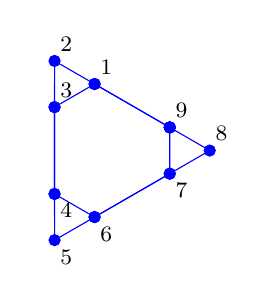
\begin{tikzpicture} 
\begin{axis}[footnotesize,font=\footnotesize
    ,axis equal image, axis lines=none ]
    \addplot[blue,mark=*,domain=40:400,samples=10
    ,nodes near coords={\quad\color{black}\ifnum\coordindex=0\else\coordindex\fi}] 
    ({cos(\x)+0.347*cos(2*\x)}
    ,{sin(\x)-0.347*sin(2*\x)});
    \addplot[blue,mark=*,samples at={40,80,160,200,280,320,40}] 
    ({cos(\x)+0.347*cos(2*\x)}
    ,{sin(\x)-0.347*sin(2*\x)});
\end{axis}
\end{tikzpicture}
\end{wrapfigure}
\begin{example} \label{eg:sier2eigp}
Recall the \idx{Sierpinski network} of \cref{eg:sier2eig} (shown to the right).
The following \(9\times9\) matrix~\(A\) encodes the network.  
Is the matrix diagonalizable?
\begin{equation*}
A=\begin{bmatrix}-3&1&1&0&0&0&0&0&1
\\1&-2&1&0&0&0&0&0&0
\\1&1&-3&1&0&0&0&0&0
\\0&0&1&-3&1&1&0&0&0
\\0&0&0&1&-2&1&0&0&0
\\0&0&0&1&1&-3&1&0&0
\\0&0&0&0&0&1&-3&1&1
\\0&0&0&0&0&0&1&-2&1
\\1&0&0&0&0&0&1&1&-3 \end{bmatrix}.
\end{equation*}

\begin{solution} 
In that example we used \script\ command \verb|[V,D]=eig(A)| to compute a matrix of eigenvectors~\verb|V| and the corresponding diagonal matrix of eigenvalues~\verb|D| where \twodp
\begin{verbatim}
V =
 -0.41  0.51 -0.16 -0.21 -0.45  0.18 -0.40  0.06  0.33
  0.00 -0.13  0.28  0.63  0.13 -0.18 -0.58 -0.08  0.33
  0.41 -0.20 -0.49 -0.42  0.32  0.01 -0.36 -0.17  0.33
 -0.41 -0.11  0.52 -0.42  0.32  0.01  0.14 -0.37  0.33
 -0.00 -0.18 -0.26  0.37 -0.22  0.51  0.36 -0.46  0.33
  0.41  0.53  0.07  0.05 -0.10 -0.51  0.33 -0.23  0.33
 -0.41 -0.39 -0.36  0.05 -0.10 -0.51  0.25  0.31  0.33
  0.00  0.31 -0.03  0.16  0.55  0.34  0.22  0.55  0.33
  0.41 -0.33  0.42 -0.21 -0.45  0.18  0.03  0.40  0.33
D =
 -5.00     0     0     0     0     0     0     0     0
     0 -4.30     0     0     0     0     0     0     0
     0     0 -4.30     0     0     0     0     0     0
     0     0     0 -3.00     0     0     0     0     0
     0     0     0     0 -3.00     0     0     0     0
     0     0     0     0     0 -3.00     0     0     0
     0     0     0     0     0     0 -0.70     0     0
     0     0     0     0     0     0     0 -0.70     0
     0     0     0     0     0     0     0     0 -0.00
\end{verbatim}
%From these we identify the following eigenspaces:
%\begin{eqnarray*}
%&&\EE_{-5}=\Span\{(-1,0,1,-1,0,1,-1,0,1)\};
%\\&&\EE_{-4.30}=\Span\left\{ \begin{bmatrix} 0.51\\-0.13\\-0.20\\-0.11\\-0.18\\0.53\\-0.39\\0.31\\-0.33 \end{bmatrix},\  \begin{bmatrix} -0.16\\0.28\\-0.49\\0.52\\-0.26\\0.07\\-0.36\\-0.03\\0.42 \end{bmatrix} \right\};
%\\&&\EE_{-3}=\Span\left\{ 
%\begin{bmatrix} -0.21\\0.63\\-0.42\\-0.42\\0.37\\0.05\\0.05\\0.16\\-0.21
%\end{bmatrix},\  
%\begin{bmatrix} -0.45\\0.13\\0.32\\0.32\\-0.22\\-0.10\\-0.10\\0.55\\-0.45
%\end{bmatrix},\ 
%\begin{bmatrix} 0.18\\-0.18\\0.01\\0.01\\0.51\\-0.51\\-0.51\\0.34\\0.18
% \end{bmatrix} \right\};
%\\&&\EE_{-0.70}=\Span\left\{ \begin{bmatrix} -0.40\\-0.58\\-0.36\\0.14\\0.36\\0.33\\0.25\\0.22\\0.03 \end{bmatrix},\  \begin{bmatrix} 0.06\\-0.08\\-0.17\\-0.37\\-0.46\\-0.23\\0.31\\0.55\\0.40 \end{bmatrix} \right\}; 
%\\&&\EE_{0}=\Span\{(1,1,1,1,1,1,1,1,1)\}.
%\end{eqnarray*}
Since matrix~\(A\) is symmetric, \script\ computes for us an orthogonal matrix~\(V\) with columns eigenvectors.
Since~\(V\) is orthogonal, its column vectors are orthonormal and hence its columns are linearly independent (\cref{thm:ortholi}).
Since there exist nine linearly independent eigenvectors, the nine column vectors of~\(V\), the matrix~\(A\) is diagonalizable.
Further, the product \(V^{-1}AV=D\) for the above diagonal matrix~\(D\) of eigenvalues in the order of the eigenvectors in~\(V\).
(Also, since \(V\)~is orthogonal, \(\tr VAV=D\).)
\aqed

\end{solution}
\end{example}





\begin{example} \label{eg:faespmp}
Recall that \cref{eg:faespm} found \idx{eigenvalue}s and corresponding \idx{eigenspace}s for various matrices.
Revisit these cases and show that none of the matrices are diagonalizable.
\begin{enumerate}
\item Matrix \(A=\begin{bmat} 3&1\\0&3 \end{bmat}\) had one eigenvalue \(\lambda=3\) with \idx{multiplicity} two and corresponding eigenspace \(\EE_3=\Span\{(1,0)\}\).
This matrix is not diagonalizable as it has only one \idx{linearly independent} eigenvector, such as~\((1,0)\) or any nonzero multiple, and it needs two to \text{be diagonalizable.}

\item Matrix \(B=\begin{bmat}-1&1&-2
\\-1&0&-1
\\0&-3&1 \end{bmat}\)
has eigenvalues  \(\lambda=-2\) (multiplicity one) and \(\lambda=1\) (multiplicity two).
The corresponding eigenspaces are \(\EE_{-2}=\Span\{(1,1,1)\}\) and \(\EE_{1}=\Span\{(-1,0,1)\}\).
Thus the matrix has only two \idx{linearly independent} eigenvectors, one from each eigenspace, and it needs three to \text{be diagonalizable.}

\item Matrix \(C=\begin{bmat}-1&0&-2
\\0&-3&2
\\0&-2&1\end{bmat}\)
has only the eigenvalue \(\lambda=-1\) with multiplicity three.
The corresponding eigenspace \(\EE_{-1}=\Span\{(1,0,0)\}\).
With only one \idx{linearly independent} eigenvector, the matrix is not diagonalizable.
\aqed

\end{enumerate}
\end{example}


\begin{example} \label{eg:fiveevp}
Use the results of \cref{eg:fiveev} to show that the following matrix is \idx{diagonalizable}:
\begin{equation*}
A=\begin{bmatrix}0&3&0&0&0
\\1&0&3&0&0
\\0&1&0&3&0
\\0&0&1&0&3
\\0&0&0&1&0\end{bmatrix}
\end{equation*}
\begin{solution} 
\cref{eg:fiveev} derived that the five eigenvalues are  \(\lambda=0,\pm\sqrt3,\pm3\)\,, all of multiplicity one.
Further, the corresponding eigenspaces are
\begin{eqnarray*}
&&\EE_0=\Span\{(9,0,-3,0,1)\},
\\&&\EE_{\pm\sqrt3}=\Span\{(-9,\mp3\sqrt3,0,\pm\sqrt3,1)\},
\\&&\EE_{\pm3}=\Span\{(9,\pm9,6,\pm3,1)\}.
\end{eqnarray*}
Here there are five linearly independent eigenvectors, one from each distinct eigenspace  (\cref{thm:indepev}).
Since \(A\) is a \(5\times5\) matrix it is thus diagonalizable.
Further, \cref{thm:gendiag} establishes that the matrix formed from the columns of the five eigenvectors is a possible matrix
\begin{equation*}
P=\begin{bmatrix} 9&-9&-9&9&9
\\0&-3\sqrt3&3\sqrt3&9&-9
\\-3&0&0&6&6
\\0&\sqrt3&-\sqrt3&3&-3
\\1&1&1&1&1
\end{bmatrix}.
\end{equation*}
(One could also scale each column of~\(P\) by a different arbitrary nonzero constant, and the diagonalization still holds.)
Lastly, \cref{thm:gendiag} establishes the diagonal matrix
\(P^{-1}AP=D=\diag(0,\sqrt3,-\sqrt3,3,-3)\) is that of the eigenvalues in the order corresponding to the eigenvectors in~\(P\).
\end{solution}
\end{example}





These examples illustrate a widely useful property.
The \(5\times 5\) matrix in \cref{eg:fiveevp} has five distinct eigenvalues whose corresponding \idx{eigenvector}s are necessarily \idx{linearly independent} (\cref{thm:indepev}) and so diagonalize the matrix (\cref{thm:gendiag}).
The \(3\times 3\) matrix in \cref{eg:trieigp} has three distinct eigenvalues whose corresponding eigenvectors are necessarily \idx{linearly independent} (\cref{thm:indepev}) and so diagonalize the matrix (\cref{thm:gendiag}).
However, the matrices of \cref{eg:sier2eigp,eg:faespmp} have \idx{repeated eigenvalue}s---eigenvalues of \idx{multiplicity} two or more---and these matrices may (\cref{eg:sier2eigp}) or may not (\cref{eg:faespmp}) be diagonalizable.
The following theorem confirms that matrices with as many \emph{distinct} eigenvalues as the \idx{size} of the matrix are \text{always diagonalizable.}






\begin{theorem} \label{thm:dlamd} 
For every \(n\times n\) \idx{square matrix}~\(A\), if~\(A\) has \(n\)~\idx{distinct eigenvalues}, then \(A\)~is \idx{diagonalizable}.
Consequently, and allowing nonreal \idx{complex eigenvalue}s, a real \idx{non-diagonalizable} matrix must be non-symmetric and must have at least one \idx{repeated eigenvalue} (an \idx{eigenvalue} with \idx{multiplicity} two or~more).
\end{theorem}
\begin{proof}  
First, let \hlist\vv n\ be eigenvectors corresponding to the \(n\)~distinct eigenvalues of matrix~\(A\).
(Recall that \cref{thm:geecp} establishes that there cannot be more than \(n\)~eigenvalues.)
As the corresponding eigenvalues are distinct, \cref{thm:indepev} establishes that these eigenvectors are linearly independent.
\cref{thm:gendiag} then establishes that the matrix~\(A\) \text{is diagonalizable.}

Second, since an \(n\times n\) matrix has \(n\)~eigenvalues, when counted accordingly to multiplicity and allowing for nonreal complex valued eigenvalues (\cref{pro:geneig}), a non-diagonalizable matrix must have at least one repeated eigenvalue.  
Further, by \cref{thm:symspec} a real symmetric matrix is always diagonalizable: hence a non-diagonalizable matrix must also \text{be non-symmetric.}
\end{proof}


\begin{example} 
From the given information, are the matrices diagonalizable?
\begin{enumerate}
\item The only \idx{eigenvalue}s of a \(4\times 4\) matrix are \(1.8\), \(-3\), \(0.4\), and~\(3.2\).
\begin{solution} 
\cref{thm:dlamd} implies the matrix must be diagonalizable.
\end{solution}

\item The only eigenvalues of a \(5\times 5\) matrix are \(1.8\), \(-3\), \(0.4\), and~\(3.2\).
\begin{solution} 
Here there are only four distinct eigenvalues of the \(5\times5\) matrix.
\cref{thm:dlamd} does not apply as the precondition that there be five distinct eigenvalues is not met: the matrix may or may not be diagonalizable---it is unknowable on this information.
\end{solution}

\item The only eigenvalues of a \(3\times 3\) matrix are \(1.8\), \(-3\), \(0.4\), and~\(3.2\).
\begin{solution} 
An error has been made in determining the eigenvalues because a \(3\times3\) matrix has at most three distinct eigenvalues (\cref{thm:geecp}).
Because of the error, we cannot answer.
\end{solution}

\end{enumerate}
\end{example}



\begin{activity}
A \(3\times3\) matrix~\(A\) depends upon a parameter~\(a\) and has \idx{eigenvalue}s \(6\), \(3-3a\)\,, and \(2+a\)\,.
For which of the following values of parameter~\(a\) may the matrix be \emph{not} diagonalizable?
\actposs[4]{\(a=4\)}{\(a=1\)}{\(a=2\)}{\(a=3\)}
Extension: what are the two other values of~\(a\) for which the matrix \emph{may not} be diagonalizable?
\end{activity}





\begin{example} 
\script\ computes the \idx{eigenvalue}s of matrix
\begin{equation*}
A=\begin{bmatrix}-1&2&-2&1&-2
\\-3&-1&-2&5&6
\\3&1&6&-2&-1
\\1&1&2&1&-1
\\7&5&-3&0&0 \end{bmatrix}
\end{equation*}
via \index{eig()@\texttt{eig()}}\verb|eig(A)| and reports them to be \twodp
\begin{verbatim}
ans =
  -3.45 + 3.50i
  -3.45 - 3.50i
   5.00
   5.00
   1.91
\end{verbatim}
Is the matrix diagonalizable?
\begin{solution} 
The matrix appears to have only four distinct eigenvalues (two of them non-real \idx{complex valued}), and so on the given information \cref{thm:dlamd} cannot determine whether the matrix is diagonalizable \text{or not.}

However, upon reporting the eigenvalues to four \idx{decimal places} we find the two eigenvalues of~\verb|5.00| \twodp\ are more precisely two separate eigenvalues of~\verb|5.0000| and~\verb|4.9961|.
Hence this matrix has five distinct eigenvalues and so \cref{thm:dlamd} implies that the matrix is diagonalizable.%
\footnote{Nonetheless, in an application where errors are significant then the matrix may be effectively \idx{non-diagonalizable}.
Such effective non-diagonalizability is indicated by poor conditioning of the matrix of eigenvectors which here has the poor \texttt{rcond} of~\(0.0004\) (\cref{pro:unisol}).}
\end{solution}
%\begin{verbatim}
%for i=1:99999,a=round(randn(5)*3); if abs(min(abs(diff(eig(a))))-3e-3)<2e-3, eig(a), break, end, end
%\end{verbatim}
\end{example}





Recall that \cref{def:eigmult} defined the \idx{multiplicity} of every eigenvalue in terms of the characteristic polynomial.
Also, the earlier \cref{def:eigsymult} identified that for every \index{symmetric matrix}\emph{symmetric} matrix the \idx{dimension} of an \idx{eigenspace}, \(\dim\EE_{\lambda_j}\), is equal to the \idx{multiplicity} of the corresponding eigenvalue~\(\lambda_j\).
However, for general non-symmetric matrices this equality between multiplicity and eigenspace dimension does not \text{necessarily hold.}


\begin{theorem} \label{thm:dimee} 
For every square matrix~\(A\), and for each \idx{eigenvalue}~\(\lambda_j\) of~\(A\), the corresponding \idx{eigenspace}~\(\EE_{\lambda_j}\) has \idx{dimension} less than or equal to the \idx{multiplicity} of~\(\lambda_j\);
that is, \(1\leq\dim\EE_{\lambda_j}\leq\text{\idx{multiplicity} of }\lambda_j\)\,.  
\end{theorem}
%\begin{comment}
%Maths I 2014 course omits any proof.
%\end{comment}
%\begin{proof} 
%Suppose \(\lambda_j\) is an eigenvalue of matrix~\(A\) and \(\dim\EE_{\lambda_j}=p<n\) (the case \(p=n\) is proved by \cref{ex:dimme}).
%Then to span \(\EE_{\lambda_j}\) there are \(p\) corresponding, linearly independent, eigenvectors \hlist\vv p\,.
%Let
%\begin{equation*}
%P=\begin{bmatrix} \vv_1&\cdots&\vv_p&\wv_{p+1}&\cdots&\wv_n \end{bmatrix}
%\end{equation*}
%be any invertible matrix with \hlist\vv p\ as its first \(p\)~columns.
%Equivalently, write as the partitioned matrix \(P=\begin{bmatrix} V&W \end{bmatrix}\) for corresponding \(n\times p\) and \(n\times(n-p)\) matrices.
%Since the columns of~\(V\) are eigenvectors corresponding to eigenvalue~\(\lambda_j\), \(AV=A\begin{bmatrix} \vv_1&\cdots&\vv_p \end{bmatrix}
%=\begin{bmatrix} A\vv_1&\cdots&A\vv_p \end{bmatrix}
%=\begin{bmatrix} \lambda_j\vv_1&\cdots&\lambda_j\vv_p \end{bmatrix}
%=\lambda_j\begin{bmatrix} \vv_1&\cdots&\vv_p \end{bmatrix}
%=\lambda_jV\).
%Partition the inverse of~\(P\) as \(P^{-1}=\begin{bmatrix} B\\C \end{bmatrix}\) for \(p\times n\) and \((n-p)\times n\) matrices~\(B\) and~\(C\), respectively.
%From this partitioning,
%\begin{eqnarray*}&&
%P^{-1}P=\begin{bmatrix} B\\C \end{bmatrix}\begin{bmatrix} V&W \end{bmatrix}
%=\begin{bmatrix} BV&BW\\CV&CW \end{bmatrix}
%\\\text{and}&&
%P^{-1}P=I_n=\begin{bmatrix} I_p&O\\O&I_{n-p} \end{bmatrix},
%\end{eqnarray*}
%so \(BV=I_p\)\,, \(BW=O\)\,, \(CV=O\), and \(CW=I_{n-p}\)\,.
%
%Now consider
%\begin{eqnarray*}
%P^{-1}AP
%&=&\begin{bmatrix} B\\C \end{bmatrix}A\begin{bmatrix} V&W \end{bmatrix}
%=\begin{bmatrix} BAV&BAW\\CAV&CAW \end{bmatrix}
%\\
%&=&\begin{bmatrix} \lambda_jBV&BAW\\\lambda_jCV&CAW \end{bmatrix}
%=\begin{bmatrix} \lambda_jI_p&BAW\\O&CAW \end{bmatrix}
%\end{eqnarray*}
%Then the characteristic polynomial of matrix~\(A\) becomes
%\begin{eqnarray*}
%&&\hspace{-1.5em}\det(A-\lambda I_n)
%\\&=&\det(PP^{-1}APP^{-1}-\lambda PP^{-1})
%\quad(\text{as }PP^{-1}=I_n)
%\\&=&\det[P(P^{-1}AP-\lambda I_n)P^{-1}]
%\\&=&\det P\det(P^{-1}AP-\lambda I_n)\det(P^{-1})
%\quad(\text{product \cref{thm:detprod}})
%\\&=&\det P\det(P^{-1}AP-\lambda I_n)\frac1{\det P}
%\quad(\text{inverse \cref{thm:detinv}})
%\\&=&\det(P^{-1}AP-\lambda I_n)
%\\&=&\det\begin{bmatrix} (\lambda_j-\lambda)I_p&BAW\\O&CAW -\lambda I_{n-p}\end{bmatrix}
%\quad(\text{by above }PAP^{-1})
%\\&=&(\lambda_j-\lambda)^p\det(CAW -\lambda I_{n-p})
%\end{eqnarray*}
%by \(p\)~successive first column expansions of the determinant (\cref{thm:letdet}).
%Because of the factor \((\lambda_j-\lambda)^p\) in the characteristic polynomial of~\(A\), the eigenvalue~\(\lambda_j\) must have multiplicity of at least~\(p=\dim\EE_{\lambda_j}\)
%(there may be more factors of \((\lambda_j-\lambda)\) hidden within \(\det(CAW -\lambda I_{n-p})\)).
%\end{proof}

\begin{comment}Reviewer comment:
It may be useful to point out that the computation actually establishes the fact that for any square matrix \(A\) and any same-size invertible matrix \(P\), the characteristic polynomials of \(A\) and \(P^{-1}AP\) are the same. (Change of basis formula, same underlying linear transformation, eigenvalues come from the lin. tranf. and not the matrix. But perhaps this is not the right place for this kind of explanation.)
\end{comment}
\begin{proof} 
Suppose \(\lambda_j\) is an eigenvalue of \(n\times n\) matrix~\(A\) and \(\dim\EE_{\lambda_j}=p<n\) (the case \(p=n\) is proved by \cref{ex:dimme}).
Because its dimension is~\(p\), the eigenspace may be spanned by \(p\)~vectors.
Then choose \(p\)~orthonormal vectors \hlist\vv p\ to span~\(\EE_{\lambda_j}\); these vectors \hlist\vv p\ are eigenvectors as they are in the eigenspace.
Let
\begin{equation*}
P=\begin{bmatrix} \vv_1&\cdots&\vv_p&\wv_{p+1}&\cdots&\wv_n \end{bmatrix}
\end{equation*}
be any orthogonal matrix with \hlist\vv p\ as its first \(p\)~columns.
Equivalently, write as the partitioned matrix \(P=\begin{bmatrix} V&W \end{bmatrix}\) for corresponding \(n\times p\) and \(n\times(n-p)\) matrices.
Since \(P\)~is orthogonal, its inverse \(P^{-1}=\tr P=\begin{bmat} \tr V\\\tr W \end{bmat}\).
Since the columns of~\(V\) are eigenvectors corresponding to eigenvalue~\(\lambda_j\), \(AV=A\begin{bmatrix} \vv_1&\cdots&\vv_p \end{bmatrix}
=\begin{bmatrix} A\vv_1&\cdots&A\vv_p \end{bmatrix}
=\begin{bmatrix} \lambda_j\vv_1&\cdots&\lambda_j\vv_p \end{bmatrix}
=\lambda_j\begin{bmatrix} \vv_1&\cdots&\vv_p \end{bmatrix}
=\lambda_jV\).

Now consider
\begin{eqnarray*}
P^{-1}AP
&=&\begin{bmatrix} \tr V\\\tr W \end{bmatrix}A\begin{bmatrix} V&W \end{bmatrix}
=\begin{bmatrix} \tr VAV&\tr VAW\\\tr WAV&\tr WAW \end{bmatrix}
\\
&=&\begin{bmatrix} \lambda_j\tr VV&\tr VAW\\\lambda_j\tr WV&\tr WAW \end{bmatrix}
=\begin{bmatrix} \lambda_jI_p&\tr VAW\\O&\tr WAW \end{bmatrix}
\end{eqnarray*}
where the last equality follows from the orthonormality of columns of \(P=\begin{bmatrix} V&W \end{bmatrix}\).
Then the characteristic polynomial of matrix~\(A\) becomes
\begin{eqnarray*}
&&\hspace{-1.5em}\det(A-\lambda I_n)
\\&=&\det(PP^{-1}APP^{-1}-\lambda PP^{-1})
\quad(\text{as }PP^{-1}=I_n)
\\&=&\det[P(P^{-1}AP-\lambda I_n)P^{-1}]
\\&=&\det P\det(P^{-1}AP-\lambda I_n)\det(P^{-1})
\quad(\text{product \cref{thm:detprod}})
\\&=&\det P\det(P^{-1}AP-\lambda I_n)\frac1{\det P}
\quad(\text{inverse \cref{thm:detinv}})
\\&=&\det(P^{-1}AP-\lambda I_n)
\\&=&\det\begin{bmatrix} (\lambda_j-\lambda)I_p&\tr VAW\\O&\tr WAW -\lambda I_{n-p}\end{bmatrix}
\quad(\text{by above }P^{-1}AP)
\\&=&(\lambda_j-\lambda)^p\det(\tr WAW -\lambda I_{n-p})
\end{eqnarray*}
by \(p\)~successive first column expansions of the determinant (\cref{thm:letdet}).
Because of the factor \((\lambda_j-\lambda)^p\) in the characteristic polynomial of~\(A\), the eigenvalue~\(\lambda_j\) must have multiplicity of at least~\(p=\dim\EE_{\lambda_j}\)---there may be more factors of \((\lambda_j-\lambda)\) hidden within \(\det(\tr WAW -\lambda I_{n-p})\).
\end{proof}



\begin{example} 
Show that the matrix \(A=\begin{bmat}0&5&6
\\-8&22&24
\\6&-15&-16 \end{bmat}\) has one \idx{eigenvalue} of \idx{multiplicity} three, and that the corresponding \idx{eigenspace} has \idx{dimension} two.
%\begin{equation*}
%A=\begin{bmatrix}0&5&6
%\\-8&22&24
%\\6&-15&-16 \end{bmatrix}
%\end{equation*}
\begin{solution} 
Find eigenvalues via the characteristic polynomial
\begin{eqnarray*}
\det(A-\lambda I)
&=&
\begin{vmatrix} -\lambda&5&6
\\-8&22-\lambda&24
\\6&-15&-16-\lambda \end{vmatrix}
\\&=&-\lambda(22-\lambda)(-16-\lambda)+5\cdot24\cdot6+6(-8)(-15)
\\&&{}-6(22-\lambda)6+\lambda24(-15)-5(-8)(-16-\lambda)
\\&\vdots&
\\&=&-\lambda^3+6\lambda^2-12\lambda+8
=-(\lambda-2)^3.
\end{eqnarray*}
This characteristic polynomial is zero only for eigenvalue \(\lambda=2\) which is of multiplicity three.

The corresponding eigenspace comes from solving \((A-\lambda I)\xv=\ov\) which here is
\begin{equation*}
\begin{bmatrix}-2&5&6
\\-8&20&24
\\6&-15&-18 \end{bmatrix}\xv=\ov.
\end{equation*}
Observe that the second row is just four times the first row, and the third row is \((-3)\)~times the first row, hence all three equations in this system are equivalent to just the one from the first row, namely \(-2x_1+5x_2+6x_3=0\)\,.
A general solution of this equation is \(x_1=\tfrac52x_2+3x_3\)\,.
That is, all solutions are \(\xv=(\tfrac52x_2+3x_3,x_2,x_3)=x_2(\tfrac52,1,0)+x_3(3,0,1)\). 
Hence all solutions form the two-dimensional eigenspace 
\(\EE_2=\Span\{(\tfrac52,1,0)\clb (-3,0,1)\}\).
\end{solution}
\end{example}



\begin{example} 
Use \script\ to find the \idx{eigenvalue}s and the \idx{dimension} of the \idx{eigenspace}s of the matrix 
\begin{equation*}
B=\begin{bmatrix} 344&-1165&-149&-1031&1065&-2816
\\90&-306&-38&-272&280&-742
\\-45&140&12&117&-115&302
\\135&-470&-70&-421&445&-1175
\\-165&555&67&493&-506&1338
\\-105&360&48&322&-335&886 \end{bmatrix}.
\end{equation*}

\begin{solution} 
In \script\ enter the matrix with
\begin{verbatim}
B=[344 -1165  -149 -1031  1065 -2816
    90  -306   -38  -272   280  -742
   -45   140    12   117  -115   302
   135  -470   -70  -421   445 -1175
  -165   555    67   493  -506  1338
  -105   360    48   322  -335   886]
\end{verbatim}
\setbox\ajrqrbox\hbox{\qrcode{% eigenspaces
B=[344 -1165  -149 -1031  1065 -2816
    90  -306   -38  -272   280  -742
   -45   140    12   117  -115   302
   135  -470   -70  -421   445 -1175
  -165   555    67   493  -506  1338
  -105   360    48   322  -335   886]
[V,D]=eig(B)
svd(V(:,1:3))
svd(V(:,4:6))
}}%
\marginajrbox%
Then \verb|[V,D]=eig(B)| computes something like the following \twodp
\begin{verbatim}
V =
  -0.19   0.19  -0.45   0.75  -0.20   0.15
  -0.38   0.38   0.12   0.26  -0.03   0.00
  -0.58   0.58   0.08  -0.00  -0.54   0.56
  -0.00  -0.00  -0.83   0.28  -0.50   0.52
   0.58  -0.58  -0.29  -0.45  -0.64   0.63
   0.38  -0.38   0.08  -0.29  -0.04   0.03
D =
   4.00      0      0      0      0      0
      0   4.00      0      0      0      0
      0      0   4.00      0      0      0
      0      0      0  -1.00      0      0
      0      0      0      0  -1.00      0
      0      0      0      0      0  -1.00
\end{verbatim}
Evidently, the matrix~\(B\) has two eigenvalues, \(\lambda=4\) and \(\lambda=-1\)\,, both of multiplicity three.
Although due to round-off error \script\ reports these with errors of about~\(10^{-5}\) (\cref{sec:reas})---possibly complex errors in which case ignore small complex parts.
For each eigenvalue that \script\ reports, the three corresponding columns of~\verb|V| contain corresponding eigenvectors.
Each set of these three eigenvectors does span the corresponding eigenspace, but are not necessarily \text{linearly independent.}
\begin{itemize}
\item For eigenvalue \(\lambda=4\) the first two columns of~\verb|V| are clearly the negative of each other, and so are essentially the same eigenvector.  
The third column of~\verb|V| is clearly not proportional to the first two columns and so is linearly independent (\cref{thm:lindeplc}).
Thus \script\ has computed only two linearly independent eigenvectors, either the first and third column, or the second and third column.
Consequently, the dimension \(\dim\EE_4=2\)\,.

One can confirm this dimensionality by computing the singular values 
of the first three columns of~\verb|V| with \index{svd()@\texttt{svd()}}\verb|svd(V(:,1:3))| to find they are \(1.4278\), \(0.9806\), and \(0.0000\).
The two nonzero singular values indicate that the dimension of the span is two (\cref{pro:ospan}).

\item For eigenvalue \(\lambda=-1\) the last three columns of~\verb|V| look linearly independent and so we suspect the eigenspace dimension \(\dim\EE_{-1}=3\)\,.

%If the dimensionality of an eigenspace is less than the multiplicity of an eigenvalue, then \script\ generally computes two columns as the same or the negative of each other (as for \(\lambda=-4\) here), so that the lower dimensionality is clearly apparent.
%However, this computed result is not guaranteed.
To confirm the dimension of this eigenspace via \cref{pro:ospan}, just compute \verb|svd(V(:,4:6))| to find that the three singular values are \(1.4136\), \(1.0001\), and \(0.0414\).
Since all three singular values are nonzero, \(\dim\EE_{-1}=3\)\,.
\end{itemize}
\end{solution}
%\begin{verbatim}
%d=diag([-1 -1 -1 4 4 4]);
%d(4,5)=1;%d(5,6)=1;;
%for i=1:999999,p=round(randn(6)*3); if min(abs(abs(det(p))-[1 2 5]))<1e-7, a=p*d*inv(p), break, end, end
%\end{verbatim}
The \script\ function \index{eig()@\texttt{eig()}}\verb|eig()| may produce for you a quite different matrix~\verb|V| of eigenvectors (possibly with complex parts). 
As discussed by \cref{sec:reas}, \idx{repeated eigenvalue}s are very sensitive, and this \idx{sensitivity} means that small variations in the hidden \script\ algorithm may produce quite large changes in the matrix~\verb|V| for repeated eigenvalues.
However, each eigenspace spanned by the appropriate columns of~\verb|V| \text{is robust.}
\end{example}

\index{diagonalizable|)}





\subsection{Solve systems of differential equations}
\label{sec:ssde}
\index{differential equation|(}
\index{system|(}

\paragraph{Population modelling}
The \idx{population modelling} seen so far (\cref{sec:ddp}) expressed the changes of the population over discrete intervals in time via discrete time equations such as \(y(t+1)=\cdots\) and \(z(t+1)=\cdots\)\,.
One such example is to describe the population numbers year by year.
The alternative is to model the changes in the population \emph{continuously} in time.
This alternative invokes and analyses differential equations.
Such continuous time, differential equation models are common for exploring the interaction between different \idx{species}, such as between humans and viruses.
Such differential equations are also common throughout engineering \text{and science.}

Let's start with a continuous time version of the \idx{population modelling} discussed at the start of this \cref{ch:gee}.
Let two \idx{species} interact continuously in time with populations \(y(t)\) and~\(z(t)\) at time~\(t\) (years).
Suppose they interact according to \idx{differential equation}s \(dy/dt=y-4z\) and \(dz/dt=-y+z\) (instead of the discrete time equations \(y(t+1)=\cdots\) and \(z(t+1)=\cdots\)).
Analogous to the start of this \cref{sec:dit}, we now ask the following question: is there a matrix transformation to new variables, the vector~\(\Yv(t)\), such that \((y,z)=P\Yv\) for some as yet unknown matrix~\(P\), where the differential equations for~\Yv\ are simple?
Equivalently, is there a different basis \(\cP=\{\pv_1,\pv_2\}\) for the \(yz\)-plane in which the differential equations for \(\Yv=[\yv]_\cP\) \text{are simple?}
\begin{itemize}
\item First, form the differential equations into a matrix-vector system:
\begin{equation*}
\begin{bmatrix} dy/dt\\dz/dt \end{bmatrix}
=\begin{bmatrix} y-4z
\\ -y+z \end{bmatrix}
=\begin{bmatrix} 1&-4\\-1& 1 \end{bmatrix}\begin{bmatrix} y\\z \end{bmatrix}.
\end{equation*}
So using vector \(\yv=(y,z)\), this system is
\begin{equation*}
\D t\yv=A\yv
\quad\text{for matrix }A=\begin{bmatrix} 1&-4\\-1& 1 \end{bmatrix}.
\end{equation*}

\item Second, let's see what happens when we transform to some, as yet unknown, new vector variable~\(\Yv(t)\) such that \(\yv=P\Yv\) for some constant invertible matrix~\(P\).
Under such a transform: \(\D t\yv=\D t{}P\Yv=P\D t\Yv\); also \(A\yv=AP\Yv\).
Hence substituting such an assumed transformation into the matrix-vector form of the differential equation leads to
\begin{equation*}
P\D t\Yv=AP\Yv\,, 
\quad\text{that is}\quad
\D t\Yv=\left(P^{-1}AP\right)\Yv.
\end{equation*}
To simplify this system for~\Yv, we diagonalize the matrix on the right-hand side.
The procedure is to choose the columns of~\(P\) to be \idx{eigenvector}s of the matrix~\(A\) (\cref{thm:gendiag}).

\item Third, find the eigenvectors of~\(A\) by hand as it is a \(2\times2\) matrix. 
Here the matrix \(A=\begin{bmat} 1&-4\\-1&1 \end{bmat}\) has \idx{characteristic polynomial} \(\det(A-\lambda I)=(1-\lambda)^2-4\)\,.
This is zero for \((1-\lambda)^2=4\)\,, that is, \((1-\lambda)=\pm2\).
Hence the \idx{eigenvalue}s \(\lambda=1\pm2=3,-1\)\,.
\begin{itemize}
\item For eigenvalue \(\lambda_1=3\) the corresponding eigenvectors satisfy
\begin{equation*}
(A-\lambda_1I)\pv_1=\begin{bmatrix} -2&-4\\-1&-2 \end{bmatrix}\pv_1=\ov\,,
\end{equation*}
with general solution \(\pv_1\propto(2,-1)\).

\item For eigenvalue \(\lambda_2=-1\) the corresponding eigenvectors satisfy
\begin{equation*}
(A-\lambda_2I)\pv_2=\begin{bmatrix} 2&-4\\-1&2 \end{bmatrix}\pv_2=\ov\,,
\end{equation*}
with general solution \(\pv_2\propto(2,1)\).
\end{itemize}
Thus setting transformation matrix 
\begin{equation*}
P=\begin{bmatrix} \pv_1&\pv_2 \end{bmatrix}
=\begin{bmatrix} 2&2\\-1&1 \end{bmatrix}
\implies \D t\Yv=\begin{bmatrix} 3&0\\0&-1 \end{bmatrix}\Yv
\end{equation*}
(every nonzero scalar multiple of the two columns of~\(P\) also work).

\item Fourth, having diagonalized the matrix, expand this diagonalized set of differential equations to write this system in terms of \idx{components} \(\Yv=(Y_1,Y_2)\): 
\begin{equation*}
\D t{Y_1}=3Y_1 \quad\text{and}\quad \D t{Y_2}=-Y_2\,.
\end{equation*}
Each of these differential equations has well-known \idx{exponential} solutions, respectively \(Y_1=c_1e^{3t}\) and \(Y_2=c_2e^{-t}\),  for every value of the constants~\(c_1\) and~\(c_2\).

\item Lastly, what does this mean for the original problem?
Recall the relation
\begin{equation*}
\begin{bmatrix} y\\z \end{bmatrix}=\yv
=P\Yv=\begin{bmatrix} 2&2\\-1&1 \end{bmatrix}
\begin{bmatrix}c_1e^{3t}\\ c_2e^{-t} \end{bmatrix}
=\begin{bmatrix} 2c_1e^{3t}+2c_2e^{-t}
\\ -c_1e^{3t}+c_2e^{-t}\end{bmatrix}.
\end{equation*}
That is, a general solution of the original system of differential equations is \(y(t)=2c_1e^{3t}+2c_2e^{-t}\) and \(z(t)=-c_1e^{3t}+c_2e^{-t}\).

\end{itemize}
The diagonalization of the matrix empowers us to solve complicated systems of differential equations as a set of simple systems.


Such a \idx{general solution} makes predictions. 
For example, suppose at time zero (\(t=0\)) the \idx{initial population} (\idx{female}) of \(y\)-animals is~\(22\) and the population of \(z\)-animals is~\(9\).
From the above general solution we then know that at time \(t=0\)
\begin{equation*}
\begin{bmatrix} 22\\9 \end{bmatrix}=
\begin{bmatrix} y(0)\\z(0) \end{bmatrix}
=\begin{bmatrix} 2c_1e^{3\cdot0}+2c_2e^{-0}
\\ -c_1e^{3\cdot0}+c_2e^{-0} \end{bmatrix}
=\begin{bmatrix} 2c_1+2c_2
\\ -c_1+c_2 \end{bmatrix}
\end{equation*}

\begin{wrapfigure}r{0pt}
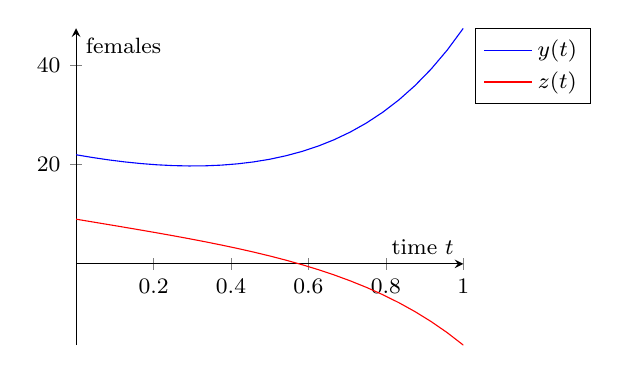
\begin{tikzpicture}
\begin{axis}[small,font=\footnotesize,domain=0:1, 
xlabel={time $t$},ylabel={females},axis lines=middle
,legend pos=outer north east]
\addplot [blue] {2*exp(3*x)+20*exp(-x)};
\addlegendentry{$y(t)$};
\addplot [red] {-exp(3*x)+10*exp(-x)};
\addlegendentry{$z(t)$};
\end{axis}
\end{tikzpicture}
\end{wrapfigure}
This determines the coefficients: \(2c_1+2c_2=22\)
and \(-c_1+c_2=9\)\,.
Adding the first to twice the second gives \(4c_2=40\)\,, that is, \(c_2=10\)\,.
Then either equation determines \(c_1=1\)\,.
Consequently, the \idx{particular solution} from this initial population is
\begin{equation*}
\begin{bmatrix} y\\z \end{bmatrix}
=\begin{bmatrix} 2\cdot1e^{3t}+2\cdot10e^{-t}
\\ -1e^{3t}+10e^{-t}\end{bmatrix}
=\begin{bmatrix} 2e^{3t}+20e^{-t}
\\ -e^{3t}+10e^{-t}\end{bmatrix}.
\end{equation*}
The graph, above-right, of this solution shows that the population of \(y\)-animals grows in time, whereas the population of \(z\)-animals crashes and becomes extinct at about time \(0.6\)~years.%
\footnote{After time \(0.6\)~years the differential equation model  and its predictions becomes meaningless as there is no biological meaning to a negative number of animals~\(z\).}


The forthcoming \cref{thm:ddtsol} confirms that the same approach solves general systems of differential equations: it is analogous to \cref{thm:dynsol} for discrete dynamics.



\begin{activity}
A given \idx{population model} is expressed as the differential equations \(dx/dt=x+y-3z\)\,, \(dy/dt=-2x+z\)\,, and \(dz/dt=-2x+y+2z\)\,.
This may be written in \idx{matrix-vector form} \(d\xv/dt=A\xv\) for vector \(\xv(t)=(x,y,z)\) and which of the following matrices?
\actposs[4]{\(\begin{bmatrix} 1&1&-3
\\-2&0&1
\\-2&1&2 \end{bmatrix}\)}
{\(\begin{bmatrix} 1&-3&1
\\-2&1&0
\\-2&2&1 \end{bmatrix}\)}
{\(\begin{bmatrix} 1&-2&2
\\0&-2&1
\\1&1&-3 \end{bmatrix}\)}
{\(\begin{bmatrix} 1&1&-3
\\0&-2&1
\\1&-2&2 \end{bmatrix}\)}
\end{activity}




\begin{theorem} \label{thm:ddtsol}
Let \(n\times n\) \idx{square matrix}~\(A\) be \idx{diagonalizable} by matrix \(P=\begin{bmatrix} \pv_1&\pv_2&\cdots&\pv_n \end{bmatrix}\) whose columns are \idx{eigenvector}s corresponding to \idx{eigenvalue}s \hlist\lambda n\ of matrix~\(A\).  
Then a \idx{general solution}~\(\xv(t)\) to the \idx{differential equation} system \(d\xv/dt=A\xv\) is the \idx{linear combination}
\begin{equation}
\xv(t)=c_1\pv_1e^{\lambda_1t}+c_2\pv_2e^{\lambda_2t}+\cdots+c_n\pv_ne^{\lambda_nt}
\label{eq:ddtsol}
\end{equation}
for arbitrary constants \hlist cn.
\end{theorem}

\begin{proof} 
First, instead of finding solutions for~\(\xv(t)\) directly, let's write the differential equations in terms of the alternate basis for~\(\RR^n\), basis \(\cP=\{\hlist\pv n\}\) (as \hlist\pv n\ are linearly independent).
That is, solve for the coordinates \(\Xv(t)=[\xv(t)]_\cP\) with respect to basis~\cP.
From \cref{thm:ssbc} recall that  \(\Xv=[\xv]_\cP\) means that \(\xv=\lincomb X\pv n=P\Xv\)\,.
Substituting this into the differential equation \(d\xv/dt=A\xv\) requires \(\D t{}(P\Xv)=A(P\Xv)\) which is the same as \(P\D t\Xv=AP\Xv\)\,.
Since matrix~\(P\) is invertible, this equation is the same as \(\D t\Xv=P^{-1}AP\Xv\)\,.
Because the columns of matrix~\(P\) are eigenvectors, the product \(P^{-1}AP\) is the diagonal matrix \(D=\diag(\hlist\lambda n)\), hence the system becomes \(\D t\Xv=D\Xv\)\,.
Because matrix~\(D\) is diagonal, this is a much simpler system of differential equations.
The \(n\)~rows of the system \(\D t\Xv=D\Xv\) are
\begin{equation*}
\D t{X_1}=\lambda_1X_1\,,\quad
\D t{X_2}=\lambda_2X_2\,,\quad \ldots,\quad
\D t{X_n}=\lambda_nX_n\,.
\end{equation*}
Each of these has general solution
\begin{equation*}
X_1=c_1e^{\lambda_1t},\quad
X_2=c_2e^{\lambda_2t},\quad \ldots,\quad
X_n=c_ne^{\lambda_nt},
\end{equation*}
where \hlist cn\ are arbitrary constants.
To rewrite this solution for the original coordinates~\xv\ use
\begin{equation*}
\xv = P\Xv
=\begin{bmatrix} \pv_1&\pv_2&\cdots&\pv_n \end{bmatrix}
\begin{bmatrix} c_1e^{\lambda_1t}
\\c_2e^{\lambda_2t}
\\\vdots
\\c_ne^{\lambda_nt} \end{bmatrix}
= c_1\pv_1e^{\lambda_1t}+c_2\pv_2e^{\lambda_2t}+\cdots+c_n\pv_ne^{\lambda_nt}
\end{equation*}
to derive the solution~\eqref{eq:ddtsol}.

\begin{comment}
Straightforward substitution is simpler, but the above reinforces the simplification through diagonalization.
\end{comment}
%First show that formula~\eqref{eq:ddtsol} is a solution by substitution into the differential equation \(d\xv/dt=A\xv\)\,: recalling from calculus that \(\D t{}e^{at}=ae^{at}\), the left-hand side
%\begin{eqnarray*}
%\D t\xv&=&c_1\pv_1\D t{}e^{\lambda_1t}+c_2\pv_2\D t{}e^{\lambda_2t}+\cdots+c_n\pv_n\D t{}e^{\lambda_nt}
%\\&=&c_1\pv_1\lambda_1e^{\lambda_1t}+c_2\pv_2\lambda_2e^{\lambda_2t}+\cdots+c_n\pv_n\lambda_ne^{\lambda_nt}\,;
%\end{eqnarray*}
%whereas the right-hand side, as \(\pv_j\) are eigenvectors,
%\begin{eqnarray*}
%A\xv&=&c_1A\pv_1e^{\lambda_1t}+c_2A\pv_2e^{\lambda_2t}+\cdots+c_nA\pv_ne^{\lambda_nt}
%\\&=&c_1\lambda_1\pv_1e^{\lambda_1t}+c_2\lambda_2\pv_2e^{\lambda_2t}+\cdots+c_n\lambda_n\pv_ne^{\lambda_nt}.
%\end{eqnarray*}
%These expressions are the same and hence formula~\eqref{eq:ddtsol} solves \(d\xv/dt=A\xv\)\,.

Second, being able to use the constants \(\cv=(\hlist cn)\) to match every given initial condition shows that formula~\eqref{eq:ddtsol} is a general solution.
Suppose the value of~\(\xv(0)\) is given.
Recalling \(e^0=1\)\,, formula~\eqref{eq:ddtsol} evaluated at \(t=0\)  requires
\begin{eqnarray*}
\xv(0)&=&c_1\pv_1e^{\lambda_10}+c_2\pv_2e^{\lambda_20}+\cdots+c_n\pv_ne^{\lambda_n0}
\\&=&c_1\pv_1+c_2\pv_2+\cdots+c_n\pv_n
=\begin{bmatrix} \pv_1&\pv_2&\cdots&\pv_n \end{bmatrix}\cv
=P\cv\,.
\end{eqnarray*}
Since matrix~\(P\) is invertible, choose constants \(\cv=P^{-1}\xv(0)\) for any given~\(\xv(0)\).
%\cref{thm:gendiag,thm:ftim3} establish that such an invertible~\(P\) exists for diagonalizable matrices~\(A\).
\end{proof}





\begin{activity}
Recall that the \idx{differential equation}s \(dy/dt=y-4z\) and \(dz/dt=-y+z\) have a \idx{general solution} \(y(t)=2c_1e^{3t}+2c_2e^{-t}\) and \(z(t)=-c_1e^{3t}+c_2e^{-t}\).
What are the values of these constants given that \(y(0)=2\) and \(z(0)=3\)?
\actposs[4]{\(c_1=-1\), \(c_2=2\)}
{\(c_1=1\), \(c_2=1\)}
{\(c_1=0\), \(c_2=-1\)}
{\(c_1=-2\), \(c_2=0\)}
\end{activity}




\begin{example} \label{eg:de3t} 
Use matrix analysis to find (by hand) a \idx{general solution} to the system of differential equations \(\D tu=-2u+2v\)\,, \(\D tv=u-2v+w\)\,, and \(\D tw=2v-2w\)\,.

\begin{solution} 
Let vector~\(\uv=(u,v,w)\), and then form the differential equations into the matrix-vector system
\begin{equation*}
\D t\uv=\begin{bmatrix} \D tu\\\D tv\\\D t w \end{bmatrix}
=\begin{bmatrix} -2u+2v\\u-2v+w\\2v-2w \end{bmatrix}
=\begin{bmatrix} -2&2&0\\1&-2&1\\0&2&-2 \end{bmatrix}
\begin{bmatrix} u\\v\\w \end{bmatrix}
=\underbrace{\begin{bmatrix} -2&2&0\\1&-2&1\\0&2&-2 \end{bmatrix}}_A\uv\,.
\end{equation*}
To use \cref{thm:ddtsol} we need eigenvalues and eigenvectors of the matrix~\(A\).
Here the characteristic polynomial of~\(A\) is, using~\eqref{eq:dets23b},
\begin{eqnarray*}
\det(A-\lambda I)&=&\det\begin{bmatrix} -2-\lambda&2&0\\1&-2-\lambda&1\\0&2&-2-\lambda \end{bmatrix}
\\&=&-(2+\lambda)^3+0+0-0+2(2+\lambda)+2(2+\lambda)
\\&=&(2+\lambda)\left[-(2+\lambda)^2+4\right]
\\&=&(2+\lambda)[-\lambda^2-4\lambda]
=-\lambda(\lambda+2)(\lambda+4).
\end{eqnarray*}
This determinant is only zero for eigenvalues \(\lambda=0,-2,-4\)\,.
\begin{itemize}
\item For eigenvalue \(\lambda=0\)\,, corresponding eigenvectors~\pv\ satisfy
\begin{equation*}
(A-0I)\pv=\begin{bmatrix} -2&2&0\\1&-2&1\\0&2&-2 \end{bmatrix}\pv=\ov\,.
\end{equation*}
The last row of this equation requires \(p_3=p_2\), and the first row requires \(p_1=p_2\).
Hence all solutions may be written as \(\pv=(p_2,p_2,p_2)\).
Choose any nonzero one, say \(\pv=(1,1,1)\).

\item For eigenvalue \(\lambda=-2\)\,, corresponding eigenvectors~\pv\ satisfy
\begin{equation*}
(A+2I)\pv=\begin{bmatrix} 0&2&0\\1&0&1\\0&2&0 \end{bmatrix}\pv=\ov\,.
\end{equation*}
The first and last rows of this equation require \(p_2=0\), and the second row requires \(p_3=-p_1\).
Hence all solutions may be written as \(\pv=(p_1,0,-p_1)\).
Choose any nonzero one, say \(\pv=(1,0,-1)\).

\item For eigenvalue \(\lambda=-4\)\,, corresponding eigenvectors~\pv\ satisfy
\begin{equation*}
(A+4I)\pv=\begin{bmatrix} 2&2&0\\1&2&1\\0&2&2 \end{bmatrix}\pv=\ov\,.
\end{equation*}
The last row of this equation requires \(p_3=-p_2\), and the first row requires \(p_1=-p_2\).
Hence all solutions may be written as \(\pv=(-p_2,p_2,-p_2)\).
Choose any nonzero one, say \(\pv=(-1,1,-1)\).

\end{itemize}
With these three distinct eigenvalues, corresponding eigenvectors are linearly independent, and so \cref{thm:ddtsol} gives a general solution of the differential equations as
\begin{equation*}
\begin{bmatrix} u\\v\\w \end{bmatrix}
=c_1\begin{bmatrix} 1\\1\\1 \end{bmatrix}e^{0t}
+c_2\begin{bmatrix} 1\\0\\-1 \end{bmatrix}e^{-2t}
+c_3\begin{bmatrix} -1\\1\\-1 \end{bmatrix}e^{-4t}.
\end{equation*}
That is, \(u(t)=c_1+c_2e^{-2t}-c_3e^{-4t}\), \(v(t)=c_1+c_3e^{-4t}\), and \(w(t)=c_1-c_2e^{-2t}-c_3e^{-4t}\) for every values of the constants~\(c_1\), \(c_2\), and~\(c_3\).
\end{solution}
\end{example}





\begin{example} 
Use the general solution derived in \cref{eg:de3t} to predict the solution of the differential equations \(\D tu=-2u+2v\)\,, \(\D tv=u-2v+w\)\,, and \(\D tw=2v-2w\) given the \idx{initial condition}s that \(u(0)=v(0)=0\) and \(w(0)=4\)\,.
\begin{solution} 
Evaluating the general solution
\begin{equation*}
\begin{bmatrix} u\\v\\w \end{bmatrix}
=c_1\begin{bmatrix} 1\\1\\1 \end{bmatrix}
+c_2\begin{bmatrix} 1\\0\\-1 \end{bmatrix}e^{-2t}
+c_3\begin{bmatrix} -1\\1\\-1 \end{bmatrix}e^{-4t}
\end{equation*}
at time \(t=0\) gives, using the initial conditions and \(e^0=1\)\,,
\begin{equation*}
\begin{bmatrix} 0\\0\\4 \end{bmatrix}
=c_1\begin{bmatrix} 1\\1\\1 \end{bmatrix}
+c_2\begin{bmatrix} 1\\0\\-1 \end{bmatrix}
+c_3\begin{bmatrix} -1\\1\\-1 \end{bmatrix}
=\begin{bmatrix} c_1+c_2-c_3\\c_1+c_3\\c_1-c_2-c_3 \end{bmatrix}.
\end{equation*}


\begin{wrapfigure}r{0pt}
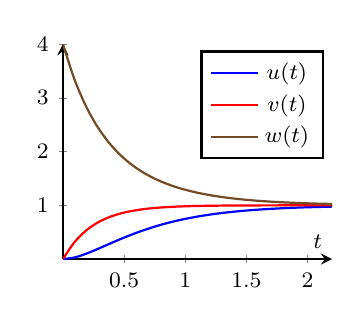
\begin{tikzpicture}
\begin{axis}[footnotesize,font=\footnotesize
,axis lines=middle,xlabel={$t$},no marks,thick
,domain=0:2.2,smooth,legend pos=north east]
\addplot+[]{1-2*exp(-2*x)+exp(-4*x)};
\addlegendentry{$u(t)$};
\addplot+[]{1-exp(-4*x)};
\addlegendentry{$v(t)$};
\addplot+[]{1+2*exp(-2*x)+exp(-4*x)};
\addlegendentry{$w(t)$};
\end{axis}
\end{tikzpicture}
\end{wrapfigure}
Solving by hand, the second row requires \(c_3=-c_1\)\,, so the first row then requires \(c_1+c_2+c_1=0\)\,, that is, \(c_2=-2c_1\)\,.
Putting both of these into the third row requires \(c_1+2c_1+c_1=4\)\,, that is, \(c_1=1\)\,.
Then \(c_2=-2\) and \(c_3=-1\)\,.
Consequently, as drawn to the right, the particular solution is 
\begin{equation*}
\begin{bmatrix} u\\v\\w \end{bmatrix}
=\begin{bmatrix} 1\\1\\1 \end{bmatrix}
-2\begin{bmatrix} 1\\0\\-1 \end{bmatrix}e^{-2t}
-\begin{bmatrix} -1\\1\\-1 \end{bmatrix}e^{-4t}
=\begin{bmatrix} 1-2e^{-2t}+e^{-4t}\\1-e^{-4t}\\1+2e^{-2t}+e^{-4t} \end{bmatrix}.
\end{equation*}
\end{solution}
\end{example}





\begin{example} 
Use \script\ to find a \idx{general solution} to the system of differential equations
\begin{eqnarray*}
&&dx_1/dt=-\tfrac12x_1-\tfrac12x_2+x_3+2x_4\,, 
\\&&dx_2/dt=-\tfrac12x_1-\tfrac12x_2+2x_3+x_4\,, 
\\&&dx_3/dt=\phantom{+2} x_1+2x_2-\tfrac12x_3-\tfrac12x_4\,,  
\\&&dx_4/dt=\phantom{+}2x_1+x_2-\tfrac12x_3-\tfrac12x_4\,.
\end{eqnarray*}
What is the \idx{particular solution} that satisfies the \idx{initial condition}s \(x_1(0)=-5\)\,, \(x_2(0)=-1\), and \(x_3(0)=x_4(0)=0\)\,?
Record your commands and give reasons.
%a=0+round(randn(1,4)*3),A=toeplitz(a([1 end:-1:2]),a),[v,d]=eig(A)
%P=[1 1 1 1;1 1 -1 -1;1 -1 -1 1;1 -1 1 -1]/2, A=P*diag(round(randn(1,4)*2))*P', [V,D]=eig(A)
\begin{solution} 
Write the system in matrix-vector form \(\D t\xv=A\xv\) for vector 
\begin{equation*}
\xv=\begin{bmatrix} x_1\\x_2\\x_3\\x_4 \end{bmatrix}
\quad\text{and matrix }
A=\begin{bmatrix} -\tfrac12 & -\tfrac12 & 1 & 2
\\-\tfrac12 & -\tfrac12 & 2 & 1
\\1 & 2 & -\tfrac12 & -\tfrac12
\\2 & 1 & -\tfrac12 & -\tfrac12 \end{bmatrix}.
\end{equation*}
Enter the matrix into \script\ and then find its eigenvalues and eigenvectors as follows
\begin{verbatim}
A=[-1/2 -1/2 1 2
 -1/2 -1/2 2 1
 1 2 -1/2 -1/2
 2 1 -1/2 -1/2]
[V,D]=eig(A)
\end{verbatim}
\setbox\ajrqrbox\hbox{\qrcode{% DEs
A=[-1/2 -1/2 1 2
 -1/2 -1/2 2 1
 1 2 -1/2 -1/2
 2 1 -1/2 -1/2]
[V,D]=eig(A)
c=V\slosh[-5;-1;0;0]
}}\marginajrbox%
\script\ tells us the eigenvectors and eigenvalues:
\begin{verbatim}
V =
  -0.5000   0.5000  -0.5000  -0.5000
  -0.5000  -0.5000   0.5000  -0.5000
   0.5000   0.5000   0.5000  -0.5000
   0.5000  -0.5000  -0.5000  -0.5000
D =
  -4.0000        0        0        0
        0  -1.0000        0        0
        0        0   1.0000        0
        0        0        0   2.0000
\end{verbatim}
Then \cref{thm:ddtsol} gives that a general solution of the differential equations is
\begin{equation*}
\xv=
c_1\begin{bmatrix} -\tfrac12\\-\tfrac12\\\tfrac12\\\tfrac12 \end{bmatrix}e^{-4t}
+c_2\begin{bmatrix} \tfrac12\\-\tfrac12\\\tfrac12\\-\tfrac12 \end{bmatrix}e^{-t}
+c_3\begin{bmatrix} -\tfrac12\\\tfrac12\\\tfrac12\\-\tfrac12 \end{bmatrix}e^{t}
+c_4\begin{bmatrix} -\tfrac12\\-\tfrac12\\-\tfrac12\\-\tfrac12 \end{bmatrix}e^{2t}.
\end{equation*}
Given the specified initial conditions at \(t=0\)\,, when all the above exponentials reduce to \(e^0=1\)\,, we just need to find the linear combination of the eigenvectors that equals the initial vector \(\xv(0)=(-5,-1,0,0)\); that is, solve \(V\cv=\xv(0)\).
In \script, after checking that \verb|rcond(V)| is the good value~\(0.25\), compute \verb|c=V\[-5;-1;0;0]| to find the vector of coefficients is \(\cv=(3,-2,2,3)\).
Hence the particular solution is
\begin{equation*}
\xv=
\begin{bmatrix} -\tfrac32\\-\tfrac32\\\tfrac32\\\tfrac32 \end{bmatrix}e^{-4t}
+\begin{bmatrix} -1\\1\\-1\\1 \end{bmatrix}e^{-t}
+\begin{bmatrix} -1\\1\\1\\-1 \end{bmatrix}e^{t}
+\begin{bmatrix} -\tfrac32\\-\tfrac32\\-\tfrac32\\-\tfrac32 \end{bmatrix}e^{2t}.
\end{equation*}
\end{solution}
\end{example}








\begin{example} \label{eg:decis2t} 
Use matrix analysis to find (by hand) a \idx{general solution} to the system of differential equations
\(\D ty=z\) and \(\D tz=-4y\)\,.
\begin{solution} 
Let vector~\(\yv=(y,z)\), and then form the differential equations into the matrix-vector system
\begin{equation*}
\D t\yv=\begin{bmatrix} \D ty\\\D tz \end{bmatrix}
=\begin{bmatrix} z\\-4y \end{bmatrix}
=\begin{bmatrix} 0&1\\-4&0 \end{bmatrix}
\begin{bmatrix} y\\z \end{bmatrix}
=\underbrace{\begin{bmatrix} 0&1\\-4&0 \end{bmatrix}}_A\yv\,.
\end{equation*}
To use \cref{thm:ddtsol} we need eigenvalues and eigenvectors of the matrix~\(A\).
Here the characteristic polynomial of~\(A\) is
\begin{equation*}
\det(A-\lambda I)=\det\begin{bmatrix} -\lambda&1\\-4&-\lambda \end{bmatrix}
=\lambda^2+4\,.
\end{equation*}
This determinant is only zero for \(\lambda^2=-4\), that is, \(\lambda=\pm2\i\) (where \(\i=\sqrt{-1}\))---a pair of complex conjugate eigenvalues.
\begin{itemize}
\item For eigenvalue \(\lambda=+2\i\) the corresponding eigenvectors~\(\pv\) satisfy
\begin{equation*}
(A-\lambda I)\pv=\begin{bmatrix} -2\i&1\\-4&-2\i \end{bmatrix}\pv
=\ov.
\end{equation*}
The second row of this matrix is \(-2\i\)~times the first row so we just need to satisfy the first row equation \(\begin{bmatrix} -2\i&1 \end{bmatrix}\pv=0\)\,.
This equation is \(-2\i p_1+p_2=0\), that is, \(p_2=2\i p_1\).
Hence all eigenvectors are of the form \(\pv=(1,2\i)p_1\)\,.
Choose any one, say \(\pv=(1,2\i)\).

\item Similarly, for eigenvalue \(\lambda=-2\i\) the corresponding eigenvectors~\(\pv\) satisfy
\begin{equation*}
(A-\lambda I)\pv=\begin{bmatrix} 2\i&1\\-4&2\i \end{bmatrix}\pv
=\ov.
\end{equation*}
The second row of this matrix is \(2\i\)~times the first row so we just need to satisfy the first row equation \(\begin{bmatrix} 2\i&1 \end{bmatrix}\pv=0\)\,.
This equation is \(2\i p_1+p_2=0\), that is, \(p_2=-2\i p_1\).
Hence all eigenvectors are of the form \(\pv=(1,-2\i)p_1\)\,.
Choose any one, say \(\pv=(1,-2\i)\).
\end{itemize}
With these two distinct eigenvalues, corresponding eigenvectors are linearly independent, and so \cref{thm:ddtsol} gives a general solution of the differential equations as
\begin{equation*}
\begin{bmatrix} y\\z \end{bmatrix}
=c_1\begin{bmatrix} 1\\2\i \end{bmatrix}e^{\i2t}
+c_2\begin{bmatrix} 1\\-2\i \end{bmatrix}e^{-\i2t}.
\end{equation*}
That is, \(y(t)=c_1e^{\i2t}+c_2e^{-\i2t}\) and \(z(t)=2\i c_1e^{\i2t}-2\i c_2e^{-\i2t}\) for all constants~\(c_1\) and~\(c_2\).
These formulas answer the exercise.
The next examples show that because of the complex exponentials, this solution describes oscillations in time~\(t\).
\end{solution}
\end{example}




\begin{example} \label{eg:decis2tb} 
Further consider \cref{eg:decis2t}.
Suppose we additionally know that \(y(0)=3\) and \(z(0)=0\)\,.  
Find the \idx{particular solution} that satisfies these two \idx{initial condition}s.
\begin{solution} 
Use the derived general solution that \(y(t)=c_1e^{\i2t}+c_2e^{-\i2t}\) and \(z(t)=2\i c_1e^{\i2t}-2\i c_2e^{-\i2t}\).
We find the constants~\(c_1\) and~\(c_2\) so that these satisfy the  conditions \(y(0)=3\) and \(z(0)=0\)\,.
Substitute \(t=0\) into the general solution to require, using \(e^0=1\)\,,
\begin{eqnarray*}
&&y(0)=3=c_1e^{\i2\cdot0}+c_2e^{-\i2\cdot0}=c_1+c_2\,,
\\&&z(0)=0=2\i c_1e^{\i2\cdot0}-2\i c_2e^{-\i2\cdot0}=2\i c_1-2\i c_2\,,
\end{eqnarray*}
The second of these equations requires \(2\i c_1=2\i c_2\)\,, that is, \(c_1=c_2\)\,.
The first, \(c_1+c_2=3\)\,, then requires that \(2c_1=3\)\,, that is, \(c_1=3/2\) and so \(c_2=3/2\)\,.
Hence the particular solution is
\begin{equation*}
y(t)=\frac32e^{\i2t}+\frac32e^{-\i2t} 
\quad\text{and}\quad
z(t)=3\i e^{\i2t}-3\i e^{-\i2t}.
\end{equation*}

\needlines6
\begin{wrapfigure}r{0pt}
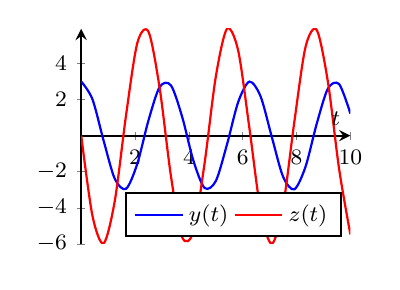
\begin{tikzpicture}
\begin{axis}[footnotesize,font=\footnotesize
,axis lines=middle,xlabel={$t$},no marks,thick
,domain=0:10,smooth,legend pos=south east,legend columns=2]
\addplot+[]{3*cos(2*deg(x))};
\addlegendentry{$y(t)$};
\addplot+[]{-6*sin(2*deg(x))};
\addlegendentry{$z(t)$};
\end{axis}
\end{tikzpicture}
\end{wrapfigure}
But recall \idx{Euler's formula} that \(e^{\i\theta}=\cos\theta+\i\sin\theta\) for every~\(\theta\).
Invoking Euler's formula the above particular solution simplifies:
\begin{eqnarray*}
y(t)&=&\frac32[\cos2t+\i\sin2t]+\frac32[\cos(-2t)+\i\sin(-2t)]
\\&=&\frac32\cos2t+\frac32\i\sin2t+\frac32\cos2t-\frac32\i\sin2t
\\&=&3\cos2t\,,
\\z(t)&=&3\i[\cos2t+\i\sin2t]-3\i[\cos(-2t)+\i\sin(-2t)]
\\&=&3\i\cos2t-3\sin2t-3\i\cos2t-3\sin2t
\\&=&-6\sin2t\,.
\end{eqnarray*}
Because \(y(t)\) and~\(z(t)\) are just trigonometric functions of~\(t\), they oscillate in time~\(t\), as illustrated above-right.
\end{solution}
\end{example}



\begin{example} \label{eg:realcis}
In a real application the \idx{complex number}s of the \idx{general solution} to \cref{eg:decis2t} are usually inconvenient.  
Instead, we typically express the solution solely in terms of real quantities as just done in the previous \cref{eg:decis2tb}.
Use \idx{Euler's formula}, that \(e^{\i\theta}=\cos\theta+\i\sin\theta\) for every~\(\theta\), to rewrite the general solution of \cref{eg:decis2t} in terms of \text{real functions.}
\begin{solution}
Here use Euler's formula in the expression for
\begin{eqnarray*}
y(t)&=&c_1e^{\i2t}+c_2e^{-\i2t}
\\&=&c_1[\cos 2t+\i\sin2t]+c_2[\cos(-2t)+\i\sin(-2t)]
\\&=&c_1\cos2t+\i c_1\sin2t +c_2\cos2t-\i c_2\sin2t
\\&=&(c_1+c_2)\cos2t +(\i c_1-\i c_2)\sin2t
\\&=&C_1\cos2t+C_2\sin2t
\end{eqnarray*}
for constants \(C_1=c_1+c_2\) and \(C_2=\i(c_1-c_2)\).
Let's view the arbitrariness in~\(c_1\) and~\(c_2\) as having been `transferred' to~\(C_1\) and~\(C_2\), then \(y(t)=C_1\cos2t+C_2\sin2t\) is a general solution to the differential equations, and is expressed purely in real factors.
In such a real form we explicitly see the oscillations in time~\(t\) through the trigonometric functions \(\cos 2t\) and~\(\sin2t\)\,.

The function \(z(t)=2\i c_1e^{\i2t}-2\i c_2e^{-\i2t}\) has a corresponding form found by replacing~\(c_1\) and~\(c_2\) in terms of the same~\(C_1\) and~\(C_2\).
From above, the constants \(C_1=c_1+c_2\) and \(C_2=\i(c_1-c_2)\).
Adding the first to \(\pm \i\)~times the second determines \(C_1-\i C_2=2c_1\) and \(C_1+\i C_2=2c_2\)\,, so that \(c_1=(C_1-\i C_2)/2\) and \(c_2=(C_1+\i C_2)/2\)\,.  
Then the expression for
\begin{eqnarray*}
z(t)&=&2\i c_1e^{\i2t}-2\i c_2e^{-\i2t}
\\&=&2\i\frac{C_1-\i C_2}2[\cos2t+\i\sin2t]
-2\i\frac{C_1+\i C_2}2[\cos2t-\i\sin2t]
\\&=&(\i C_1+C_2)[\cos2t+\i\sin2t]
+(-\i C_1+C_2)[\cos2t-\i\sin2t]
\\&=&\i C_1\cos2t-C_1\sin2t+C_2\cos2t+\i C_2\sin2t
\\&&{}
-\i C_1\cos2t-C_1\sin2t+C_2\cos2t-\i C_2\sin2t
\\&=&-2C_1\sin2t+2C_2\cos2t\,.
\end{eqnarray*}
That is, the corresponding general solution \(z(t)=-2C_1\sin2t+2C_2\cos2t\) is now also expressed in real factors.
\end{solution}
\end{example}




\begin{OmitV1}
\begingroup
\def\temp#1{\begin{tikzpicture}
\def\ugh{\ifnum0=#1 axis x line=none
\else axis x line=middle,xlabel={$x$},xtick={0}\fi}
\begin{axis}[footnotesize,font=\footnotesize
, axis y line=none,smooth,legend pos=south west
,domain=0:5.5,samples=40,axis equal,xmax=2,\ugh]
\addplot+[thick,no marks] ({2*x-cos(x*360)-12},{sin(x*360)});
\addlegendentry{spring $k$};
\addplot+[only marks,mark=*,mark size=1ex] coordinates {(0,0)};
\addlegendentry{mass $m$};
\end{axis}
\end{tikzpicture}}
\needlines5
\begin{wrapfigure}r{0pt} \temp0 \end{wrapfigure}
\begin{example}[oscillating applications] \label{eg:sprmas}
A huge variety of vibrating systems are analogous to the basic \idx{oscillation}s of a mass on a spring, 
illustrated schematically to the right.
The mass generally oscillates to and fro.  
Describe such a system mathematically with two differential equations, and solve the differential equations to confirm \text{it oscillates.}

\needlines5
\begin{solution} 
\begin{wrapfigure}r{0pt} \temp1 \end{wrapfigure}
At every time~\(t\), let the position of the mass relative to its rest position be denoted by~\(x(t)\): that is, we put an \(x\)-axis on the picture with \(x=0\) where the mass would stay at rest, as illustrated.
At every time~\(t\) let the mass be moving with velocity~\(v(t)\) (positive to the right, negative to the left).
Then we know one differential equation, that \(\D tx=v\).

\idx{Newton's law}, that \(\text{mass}\times\text{acceleration}=\text{force}\), provides another differential equation.
Here the mass is denoted by~\(m\), and the acceleration is~\(\D tv\).
The force on the mass comes from the spring: typically the force by the spring is proportional to the stretching of the spring, namely to~\(x\).
Different springs give different strength forces so let's denote the constant of proportionality by~\(k\)---a constant that differs depending upon the spring.
Then the force is~\(-kx\) as springs try to pull\slash push the mass back towards \(x=0\)\,.
Consequently Newton's law gives us the differential equation, \(m\D tv=-kx\)\,.  
Divide by mass~\(m\) and the differential equation is \(\D tv=-\frac kmx\)\,.

Write these two differential equations together as a matrix-vector system: 
\begin{equation*}
\begin{bmatrix} \D tx\\\D tv \end{bmatrix}
=\begin{bmatrix} v\\-\frac kmx \end{bmatrix},
\quad\text{that is,}\quad
\D t{}\begin{bmatrix} x\\v \end{bmatrix}
=\begin{bmatrix} 0&1\\-\frac km&0 \end{bmatrix}\begin{bmatrix} x\\v \end{bmatrix}.
\end{equation*}
\cref{thm:ddtsol} asserts a general solution comes from the eigenvalues and eigenvectors of the matrix.
\begin{itemize}
\item Here the characteristic polynomial of the matrix is
\begin{equation*}
\det\begin{bmatrix} -\lambda&1\\-\frac km&-\lambda \end{bmatrix}
=\lambda^2+\frac km\,.
\end{equation*}
This polynomial is zero only when the eigenvalues \(\lambda=\pm\sqrt{-k/m}=\pm \i\sqrt{k/m}\)\,: these are a complex conjugate pair of pure imaginary eigenvalues.

\item  The corresponding eigenvectors~\pv\ satisfy
\begin{equation*}
\begin{bmatrix} \mp \i\sqrt{k/m}&1\\- k/m&\mp \i\sqrt{k/m} \end{bmatrix}
\pv=\ov.
\end{equation*}
The two rows of this equation are satisfied by the corresponding eigenvectors \(\pv\propto (1,\pm \i\sqrt{k/m})\).
\end{itemize}
Then a general solution to the system of differential equations is
\begin{equation*}
\begin{bmatrix} x\\v \end{bmatrix}
=c_1\begin{bmatrix} 1\\\i\sqrt{k/m} \end{bmatrix}e^{\i\sqrt{k/m}t}
+c_2\begin{bmatrix} 1\\-\i\sqrt{k/m} \end{bmatrix}e^{-\i\sqrt{k/m}t}.
\end{equation*}
This formula shows that the mass on the spring generally oscillates as the complex exponentials are oscillatory.

However, in real applications we usually prefer a real algebraic expression.
Just as in \cref{eg:realcis}, we make the above formula real by changing from (complex) arbitrary constants~\(c_1\) and~\(c_2\) to new (real) arbitrary constants~\(C_1\) and~\(C_2\) where \(c_1=(C_1-\i C_2)/2\) and \(c_2=(C_1+\i C_2)/2\).
Substitute these relations into the above general solution, and using Euler's formula, gives that the position
\begin{eqnarray*}
x(t)&=&c_1e^{\i\sqrt{k/m}t}+c_2e^{-\i\sqrt{k/m}t}
\\&=&\frac{C_1-\i C_2}2\big[\cos(\sqrt{k/m}t)+\i\sin(\sqrt{k/m}t)\big]
+\frac{C_1+\i C_2}2\big[\cos(\sqrt{k/m}t)-\i\sin(\sqrt{k/m}t)\big]
\\&=&
\frac{C_1}2\cos(\sqrt{k/m}t)+\i\frac{C_1}2\sin(\sqrt{k/m}t)
-\i\frac{C_2}2\cos(\sqrt{k/m}t)+\frac{C_2}2\sin(\sqrt{k/m}t)
\\&&{}
+\frac{C_1}2\cos(\sqrt{k/m}t)-\i\frac{C_1}2\sin(\sqrt{k/m}t)
+\i\frac{C_2}2\cos(\sqrt{k/m}t)+\frac{C_2}2\sin(\sqrt{k/m}t)
\\&=&C_1\cos(\sqrt{k/m}t)+C_2\sin(\sqrt{k/m}t).
\end{eqnarray*}
For every value of the arbitrary constants~\(C_1\) and~\(C_2\), this formula describes the position~\(x(t)\) of the mass as purely real oscillations in time.
Similarly for the velocity~\(v(t)\) (\cref{ex:sprmas}).
\end{solution}
\end{example}
\endgroup
\end{OmitV1}




\index{differential equation|)}
\index{system|)}



\begin{comment}
Probable section includes Cayley--Hamilton theorem: recall \cref{sec:mpmev}, compute powers of matrices, then C-H.
Other applications include Markov chains.

Possibly develop a little more theory on similarity of matrices and coordinate transform of matrices.  Then Jordan form and solving non-diagonalizable systems of differential equations.

Possibly something on {Emergent quasi-stationary dynamics of metastable states} but perhaps done in 7.1.2--3. (Can one have too many buzz-words?)
\end{comment}















\sectionExercises


\begin{exercise} \label{ex:whichp} 
Which of the following matrices diagonalize the matrix \(Z=\begin{bmat} 7&12\\-2&-3 \end{bmat}\)?  
Show your working.
%\begin{verbatim}
%n=2
%for i=1:9999,P=0+round(randn(n)*2);if abs(det(P))==1,break,end,end
%P=P,D=diag(round(randn(1,n)*2)),A=round(P*D*inv(P))
%\end{verbatim}
\begin{Parts}
\item \(P_{\alph{enumii}}=\begin{bmatrix} -2&3\\1&-1 \end{bmatrix}\)
\answer{yes}

\item \(P_{\alph{enumii}}=\begin{bmatrix} 3&-2\\-1&1 \end{bmatrix}\)
\answer{yes}

\item \(P_{\alph{enumii}}=\begin{bmatrix} 1&-1\\-2&3 \end{bmatrix}\)
\answer{no}

\item \(P_{\alph{enumii}}=\begin{bmatrix} 1&3\\1&2 \end{bmatrix}\)
\answer{no}

\item \(P_{\alph{enumii}}=\begin{bmatrix} 4&3\\-2&-1 \end{bmatrix}\)
\answer{yes}

\item \(P_{\alph{enumii}}=\begin{bmatrix} -2&3\\2&-2 \end{bmatrix}\)
\answer{no}

\item \(P_{\alph{enumii}}=\begin{bmatrix} -1&1\\3&-2 \end{bmatrix}\)
\answer{no}

\item \(P_{\alph{enumii}}=\begin{bmatrix} 3&1\\2&1 \end{bmatrix}\)
\answer{no}

\end{Parts}
\end{exercise}



\begin{exercise} \label{ex:whichps} 
Redo \cref{ex:whichp} by finding which matrices~\(P_a,\ldots,P_h\) diagonalize each of the following matrices.
\begin{Parts}
\item \(\eAii=\begin{bmatrix} 5&12\\-2&-5 \end{bmatrix}\)
\item \(\eAii=\begin{bmatrix} -3&-12\\2&7 \end{bmatrix}\)
\item \(\eAii=\begin{bmatrix} -1&-1\\6&4 \end{bmatrix}\)
\item \(\eAii=\begin{bmatrix} 4&6\\-1&-1 \end{bmatrix}\)
\end{Parts}
\end{exercise}




\begin{exercise}  
Following \cref{eg:diagonaliseb}, prove that for every scalar~\(k\) the matrix \(\begin{bmat} k&1\\0&k \end{bmat}\) is not diagonalizable.
\end{exercise}




\begin{exercise}  
In each of the following cases, you are given three \idx{linearly independent} \idx{eigenvector}s and corresponding \idx{eigenvalue}s for some \(3\times3\) matrix~\(A\).
Write down three different matrices~\(P\) that diagonalize the matrix~\(A\), and for each, write down the corresponding \idx{diagonal matrix} \(D=P^{-1}AP\).
\begin{enumerate}
\item \(\lambda_1=-1\), \(\pv_1=(3,2,-1)\);
\(\lambda_2=1\), \(\pv_2=(-4,-2,2)\);
\(\lambda_3=3\), \(\pv_3=(-1,0,2)\).

\item \(\lambda_1=-1\), \(\pv_1=( 2,1,2)\);
\(\lambda_2=-1\), \(\pv_2=(0,3,1)\);
\(\lambda_3=2\), \(\pv_3=(4,-2,-2)\).

\item \(\lambda_1=1\), \(\pv_1=(3,-7,2)\);
\(\lambda_2=-2\), \(\pv_2=(-4,-5,1)\);
\(\lambda_3=4\), \(\pv_3=(1,2,3)\).

\begin{OmitV1}
\item \(\lambda_1=3\), \(\pv_1=(2,-3,0)\);
\(\lambda_2=1\), \(\pv_2=(-1,2,-6)\);
\(\lambda_3=-4\), \(\pv_3=(-2,-1,-3)\).
\end{OmitV1}

\end{enumerate}
\end{exercise}





\begin{exercise}  
From the given information, are each of the matrices \idx{diagonalizable}?  
Give reasons.
\begin{enumerate}
\item The only eigenvalues of a \(2\times2\) matrix are \(2.2\) and~\(0.1\).
\answer{yes}

\item The only eigenvalues of a \(4\times4\) matrix are \(2.2\), \(1.9\), \(-1.8\), and~\(-1\).
\answer{yes}

\item The only eigenvalue of a \(2\times2\) matrix is~\(0.7\).
\answer{unknown}

\item The only eigenvalues of a \(6\times6\) matrix are \(-1.6\), \(0.3\), \(0.1\), and~\(-2.3\).
\answer{unknown}

\begin{OmitV1}
\item The only eigenvalues of a \(5\times5\) matrix are \(-1.7\), \(1.4\), \(1.3\), \(2.4\), \(0.5\), and~\(-2.3\).
\answer{error}

\item The only eigenvalues of a \(6\times6\) matrix are \(1.2\), \(-0.9\), \(-0.8\), \(2.2\), \(0.2\), and~\(-0.2\).
\answer{yes}

\item The \script\ function \verb|eig(A)| returns the result
\begin{verbatim}
ans =
   2.6816
  -0.1445
   0.0798
   0.3844
\end{verbatim}
\answer{yes}
\end{OmitV1}

\item The \script\ function \verb|eig(A)| returns the result
\begin{verbatim}
ans =
   3.0821 + 0.0000i
  -2.7996 + 0.0000i
  -0.7429 + 1.6123i
  -0.7429 - 1.6123i
\end{verbatim}
\answer{yes}

\item The \script\ function \verb|eig(A)| returns the result
\begin{verbatim}
ans =
  -1.0000
   1.0000
   2.0000
  -1.0000
\end{verbatim}
\answer{unknown}

\end{enumerate}
\end{exercise}




\begin{exercise}  
For each of the following \(3\times3\) matrices, show with hand algebra that each matrix has one \idx{eigenvalue} of \idx{multiplicity} three, and then determine the \idx{dimension} of the corresponding \idx{eigenspace}.
Also compute the eigenvalue and eigenvectors with \script: comment on any limitations in the computed `eigenvalues' and `eigenvectors'.
%\begin{verbatim}
%d=eye(3)*round(randn)+[0 round(rand) 0;0 0 round(rand); 0 0 0], for i=1:99999,p=round(randn(3)*3); if abs(det(p))==1, a=round(p*d*inv(p))+0, break, end, end, [v,d]=eig(a)
%\end{verbatim}
\begin{Parts}
\item \(\eAii=\begin{bmatrix} 2 & 0 & 0
\\0 & 2 & 0
\\0 & 0 & 2 \end{bmatrix}\)
\answer{\(\lambda=2\), three; all good}

\item \(\eAii=\begin{bmatrix} 2 & 1 & -2
\\-8 & -4 & 8
\\-2 & -1 & 2 \end{bmatrix}\)
\answer{\(\lambda=0\), two; errors~\(10^{-8}\) and two  eigenvectors effectively the same}

\item \(\eAii=\begin{bmatrix} -2 & 1 & 0
\\0 & -2 & 0
\\0 & 1 & -2 \end{bmatrix}\)
\answer{\(\lambda=-2\), two; not lin.~indep.}

\item \(\eAii=\begin{bmatrix} 7 & 1 & 22
\\-6 & -1 & -20
\\-1 & 0 & -3 \end{bmatrix}\)
\answer{\(\lambda=1\), one; errors~\(10^{-5}\), all three eigenvectors effectively the same}

\begin{OmitV1}
\item \(\eAii=\begin{bmatrix} 3 & 5 & -1
\\-4 & -6 & 1
\\-5 & -6 & 0 \end{bmatrix}\)
\answer{\(\lambda=-1\), one; errors~\(10^{-6}\), all three eigenvectors \(\pm\)same}

\item \(\eAii=\begin{bmatrix} -6 & -5 & 3
\\-4 & -7 & 3
\\-12 & -15 & 7 \end{bmatrix}\)
\answer{\(\lambda=0\), two; errors~\(10^{-8}\) and two  eigenvectors effectively the same}
\end{OmitV1}

\item \(\eAii=\begin{bmatrix} -3 & 2 & 7
\\2 & -3 & -9
\\-1 & 1 & 3 \end{bmatrix}\)
\answer{\(\lambda=-1\), one;  errors~\(10^{-6}\), all three eigenvectors \(\pm\)same}

\item \(\eAii=\begin{bmatrix} -1 & 0 & 0
\\0 & -1 & 0
\\0 & 0 & -1 \end{bmatrix}\)
\answer{\(\lambda=-1\), three; all good}


\end{Parts}
\end{exercise}







\begin{exercise} \label{ex:dimme} 
For a given \(n\times n\) square matrix~\(A\), suppose \(\lambda_1\) is an \idx{eigenvalue} with \(n\)~corresponding \idx{linearly independent} \idx{eigenvector}s \hlist\pv n\,.  
Adapt parts of the proof of \cref{thm:dimee} to prove that the \idx{characteristic polynomial} of matrix~\(A\) is \(\det(A-\lambda I)=(\lambda_1-\lambda)^n\). 
Then deduce that \(\lambda_1\)~is the only eigenvalue of~\(A\), and is of \idx{multiplicity}~\(n\).
\end{exercise}




\begin{exercise}  
For each of the following matrices, use \script\ to find the \idx{eigenvalue}s, their \idx{multiplicity}, and the \idx{dimension} of the \idx{eigenspace}s.  
Give reasons (remember computational error).
%\begin{verbatim}
%d=0+round(randn(1,2)*2);
%d=diag([d(1) d(1) d(1) d(2) d(2)]);
%d([2 6 8 12 20 24])=0+round(rand(6,1)*0.75).*[-1;1;-1;1;-1;1]
%for i=1:99999,p=round(randn(5)*3); if min(abs(abs(det(p))-[1 2 5]))<1e-7, a=p*d*inv(p), break, end, end,[V,D]=eig(a)
%\end{verbatim}
\begin{enumerate}
\item \(\eAii=\begin{bmatrix} -30.5 & 25.5 & 22 & -5 & -48.5
\\-111 & 88 & 76 & -20 & -173
\\87.5 & -70.5 & -61 & 16 & 136.5
\\51 & -43 & -36 & 9 & 81
\\-4.5 & 2.5 & 2 & -1 & -6.5 \end{bmatrix}\)
\setbox\ajrqrbox\hbox{\qrcode{% eig
A=[-30.5 25.5 22 -5 -48.5
 -111 88 76 -20 -173
 87.5 -70.5 -61 16 136.5
 51 -43 -36 9 81
 -4.5 2.5 2 -1 -6.5]
}}\marginajrbox%
\answer{\(\lambda=1\) twice, \(\dim\EE_{1}=1\); \(\lambda=-1\) thrice, \(\dim\EE_{-1}=2\)}

\begin{OmitV1}
\item \(\eAii=\begin{bmatrix} 2929 & 1140 & -1359 & 2352 & 406
\\-2441 & -950 & 1132 & -1960 & -338
\\-1070 & -416 & 495 & -858 & -148
\\-2929 & -1140 & 1359 & -2352 & -406
\\-895 & -347 & 412 & -715 & -124 \end{bmatrix}\)
\setbox\ajrqrbox\hbox{\qrcode{% eig
A=[2929 1140 -1359 2352 406
 -2441 -950 1132 -1960 -338
 -1070 -416 495 -858 -148
 -2929 -1140 1359 -2352 -406
 -895 -347 412 -715 -124]
}}\marginajrbox%
\answer{\(\lambda=-1\) twice, \(\dim\EE_{-1}=1\); \(\lambda=0\) thrice, \(\dim\EE_{0}=2\)}

\item \(\eAii=\begin{bmatrix} -168 & 115 & 305 & -120 & 70
\\-4710 & 3202 & 8510 & -3360 & 1990
\\450 & -305 & -813 & 320 & -190
\\-4545 & 3090 & 8205 & -3243 & 1920
\\-2415 & 1640 & 4355 & -1720 & 1017 \end{bmatrix}\)
\setbox\ajrqrbox\hbox{\qrcode{% eig
A=[-168 115 305 -120 70
 -4710 3202 8510 -3360 1990
 450 -305 -813 320 -190
 -4545 3090 8205 -3243 1920
 -2415 1640 4355 -1720 1017]
}}\marginajrbox%
\answer{\(\lambda=2\) twice, \(\dim\EE_{2}=2\); \(\lambda=-3\) thrice, \(\dim\EE_{-3}=3\)}
\end{OmitV1}

\item \(\eAii=\begin{bmatrix} -8 & 744 & -564 & 270 & 321
\\1 & -43 & 33 & -15 & -19
\\1 & 29 & -21 & 12 & 12
\\5 & -431 & 327 & -156 & -186
\\-5 & 535 & -405 & 195 & 231 \end{bmatrix}\)
\setbox\ajrqrbox\hbox{\qrcode{% eig
A=[-8 744 -564 270 321
 1 -43 33 -15 -19
 1 29 -21 12 12
 5 -431 327 -156 -186
 -5 535 -405 195 231]
}}\marginajrbox%
\answer{\(\lambda=0\) twice, \(\dim\EE_{0}=2\); \(\lambda=1\) thrice, \(\dim\EE_{1}=2\)}

\item \(\eAii=\begin{bmatrix}15.6 & 31.4 & -11.6 & -14.6 & -10.6
\\-16.6 & -32.4 & 11.6 & 14.6 & 10.6
\\33.6 & 56.4 & -19.6 & -27.6 & -15.6
\\38.6 & 75.4 & -28.6 & -35.6 & -26.6
\\-122 & -226 & 82 & 106 & 73 \end{bmatrix}\)
\setbox\ajrqrbox\hbox{\qrcode{% eig
A=[15.6 31.4 -11.6 -14.6 -10.6
 -16.6 -32.4 11.6 14.6 10.6
 33.6 56.4 -19.6 -27.6 -15.6
 38.6 75.4 -28.6 -35.6 -26.6
 -122 -226 82 106 73]
}}\marginajrbox%
\answer{\(\lambda=2\) twice, \(\dim\EE_{2}=1\); \(\lambda=-1\) thrice, \(\dim\EE_{-1}=3\)}

\item \(\eAii=\begin{bmatrix}-208 & 420 & -518 & 82 & 264
\\655 & -1336 & 1642 & -260 & -838
\\229 & -467 & 574 & -91 & -294
\\-171 & 348 & -428 & 66 & 218
\\-703 & 1431 & -1760 & 279 & 896 \end{bmatrix}\)
\setbox\ajrqrbox\hbox{\qrcode{% eig
A=[-208 420 -518 82 264
 655 -1336 1642 -260 -838
 229 -467 574 -91 -294
 -171 348 -428 66 218
 -703 1431 -1760 279 896]
}}\marginajrbox%
\answer{\(\lambda=-1\pm \i\) once each, \(\dim\EE_{-1\pm \i}=1\); \(\lambda=-2\) thrice, \(\dim\EE_{-2}=2\)}

\end{enumerate}
\end{exercise}






\begin{exercise}  
For each of the following systems of differential equations, find \idx{eigenvalue}s and \idx{eigenvector}s to derive a \idx{general solution} of the system of differential equations.  Show your working.
%\begin{verbatim}
%n=3,d=diag(0+round(randn(1,n)*(5-n)));for i=1:99999,p=round(randn(n)*3); if min(abs(abs(det(p))-[1 2 5 10]))<1e-7, a=round(p*d*inv(p)*100)/100, break, end, end,[V,D]=eig(a),V*diag(1./max(abs(V)))
%\end{verbatim}

\begin{Parts}
\item \(\D tx=x-1.5y\), \(\D ty=4x-4y\)
\answer{\((x,y)=c_1(3,4)e^{-t}+c_2(1,2)e^{-2t}\)}

\item \(\D tx=x\), \(\D ty=-12x+5y\)
\answer{\((x,y)=c_1(0,1)e^{5t}+c_2(1,3)e^{t}\)}

\item \(\D tx=7x-3y\)
\answer{Not possible: only one equation for two unknowns.}

\begin{OmitV1}
\item \(\D tu=2.8u-3.6v\), \(\D tv=-0.6u+2.2v\)
\answer{\((u,v)=c_1(3,-1)e^{4t}+c_2(2,1)e^{t}\)}

\item \(\D tp=14p+16q\), \(\D tq=-8p-10q\)
\answer{\((p,q)=c_1(2,-1)e^{6t}+c_2(-1,1)e^{-2t}\)}

\item \(\D tx=6.5x-0.6y-5.7z\), \(\D ty=-3x+4.4y+7.8z\)%, \(\D tz=1.5x-4.2y-7.9z\)
\answer{Not possible: only two equations for three unknowns.}

\item \(\D tx=-31x+26y-24z\), \(\D ty=-48x+39y-36z\), \(\D tz=-14x+10y-9z\)
\answer{\((x,y,z)=c_1(3,3,-1)e^{3t}+c_2(1,2,1)e^{-3t}+c_3(1,3,2)e^{-t}\)}
\end{OmitV1}

\item \(\D tx=0.2x+1.2z\), \(\D ty=-x\), \(\D tz=1.8x+0.8z\)
\answer{\((x,y,z)=c_1(0,1,0) +c_2(1,1,-1)e^{-t} +c_3(-2,1,3)e^{2t}\)}

\item \(\D tu=4.5u+7.5v+7.5w\), \(\D tv=3u+4v+5w\), \(\D tw=-7.5u-11.5v-12.5w\)
\answer{\((u,v,w)=c_1(-1,-1,2)e^{-3t} +c_2(-5,0,3) +c_3(0,1,-1)e^{-t}\)}

\item \(\D tp=-13p+30q+6r\), \(\D tq=-32p+69q+14r\), \(\D tr=125p-265q-54r\)
\answer{\((p,q,r)=c_1(2,2,-5)e^{2t}+c_2(3,1,2)e^{t}+c_3(0,-1,5)e^{-t}\)}

\end{Parts}
\end{exercise}





\begin{exercise}  
In each of the following, a general solution to a differential equation is given.  
Find the \idx{particular solution} that satisfies the specified \idx{initial condition}s.
Show your working.
\begin{enumerate}
\item \((x,y)=c_1(0,1)e^{-t}+c_2(1,3)e^{2t}\) where \(x(0)=2\) and \(y(0)=1\)
\answer{\((x,y)=-5(0,1)e^{-t}+2(1,3)e^{2t}\)}

\item \((x,y)=c_1(0,1)e^{-2t}+c_2(1,3)e^{t}\) where \(x(0)=0\) and \(y(0)=2\)
\answer{\((x,y)=(0,2)e^{-2t}\)}

\begin{OmitV1}
\item \(x=3c_1e^t+c_2e^{-t}\), \(y=5c_1e^t+2c_2e^{-t}\) where \(x(0)=0\) and \(y(0)=2\)
\answer{\(x=-6e^t+6e^{-t}\), \(y=-10e^t+12e^{-t}\)}

\item \(x=3c_1e^t+c_2e^{2t}\), \(y=5c_1e^t+2c_2e^{2t}\) where \(x(0)=1\) and \(y(0)=3\)
\answer{\(x=-3e^t+4e^{2t}\), \(y=-5e^t+8e^{2t}\)}
\end{OmitV1}

\item \((x,y,z)=c_1(0,0,1) +c_2(1,-1,1)e^{2t} +c_3(-2,3,1)e^{-2t}\) where \(x(0)=3\), \(y(0)=-4\), and \(z(0)=0\)
\answer{\((x,y,z)=(1,-1,1)e^{2t} +(2,-3,-1)e^{-2t}\)}

\item \((x,y,z)=c_1(0,0,1)e^{-3t} +c_2(1,-1,1) +c_3(-2,3,1)e^{-t}\) where \(x(0)=3\), \(y(0)=-4\), and \(z(0)=2\)
\answer{\((x,y,z)=(0,0,2)e^{-3t} +(1,-1,1) +(2,-3,-1)e^{-t}\)}

\end{enumerate}
\end{exercise}







\begin{exercise}  
For each of the following systems of differential equations, use \script\ to find \idx{eigenvalue}s and \idx{eigenvector}s, and hence derive a \idx{general solution} of the system of differential equations.  
Record your working.
%\begin{verbatim}
%n=4,d=diag(0+round(randn(1,n)*10)/10); if rand<0.5,d(1:2,1:2)=[d(1) -d(2,2);d(2,2) d(1)],end,
%for i=1:99999,p=round(randn(n)*3); if min(abs(abs(det(p))-[1]))<1e-7, a=round(p*d*inv(p)*1e4)/1e4, break, end, end,
%[V,D]=eig(a),vd=num2str(V',2),dd=num2str(D',2)
%\end{verbatim}

\begin{enumerate}
\item \(\begin{array}{l} 
\D t{x_1}= 15.8x_1 +17.1x_2 -119.7x_3 +153.9x_4\,,\\
\D t{x_2}= 1.4x_1 +0.1x_2 +12.9x_3 -17.1x_4\,,\\
\D t{x_3}= 6.2x_1 +6.2x_2 -43x_3 +57.6x_4\,,\\
\D t{x_4}= 3.4x_1 +3.4x_2 -25x_3 +34x_4\,.
\end{array}\)
\setbox\ajrqrbox\hbox{\qrcode{% DE
A=[15.8 17.1 -119.7 153.9
 1.4 0.1 12.9 -17.1
 6.2 6.2 -43.0 57.6
 3.4 3.4 -25.0 34.0 ]
}}\marginajrbox%
\answer{\twodp\ \(\xv
=c_1(0.71,-0.71,0,0)e^{-1.3t} 
+c_2(-0.63,-0.63,-0.42,-0.21)e^{4.4t} 
+c_3(0,0.64,0.64,0.43)e^{1.6t} 
+c_4(-0.82,0.41,0.41)e^{2.2t}\)}

\item \(\begin{array}{l} 
\D t{x_1}= -12.2x_1 +53.7x_2 +50.1x_3 -22.8x_4\,,\\
\D t{x_2}= 0.6x_1 -2.3x_2 -2.7x_3 +1.2x_4\,,\\
\D t{x_3}= -20.4x_1 +93.8x_2 +90.2x_3 -40.8x_4\,,\\
\D t{x_4}= -38.2x_1 +177.9x_2 +170.7x_3 -77.2x_4\,.
\end{array}\)
\setbox\ajrqrbox\hbox{\qrcode{% DE
A=[ -12.2 53.7 50.1 -22.8
 0.6 -2.3 -2.7 1.2
 -20.4 93.8 90.2 -40.8
 -38.2 177.9 170.7 -77.2 ]
}}\marginajrbox%
\answer{\twodp\ \(\xv
=c_1(0.63,0.63,-0.42,0.21)e^{0.5t} 
+c_2(-0.23,-0.23,-0.23,-0.92)e^{0.4t} 
+c_3(0.64,0,0.43,0.64)e^{-1.6t} 
+c_4(-0.89,0,0,0.45)e^{0.8t}\)}

\item \(\begin{array}{l} 
\D t{x_1}= x_1 +29.4x_2 -3.2x_3 -12.9x_4\,,\\
\D t{x_2}= 1.4x_1 -38.4x_2 +5.6x_3 +18.2x_4\,,\\
\D t{x_3}= 2.3x_1 -80.3x_2 +12.3x_3 +36.7x_4\,,\\
\D t{x_4}= 2.4x_1 -65x_2 +9.2x_3 +31.1x_4\,.
\end{array}\)
\setbox\ajrqrbox\hbox{\qrcode{% DE
A=[ 1.0 29.4 -3.2 -12.9
 1.4 -38.4 5.6 18.2
 2.3 -80.3 12.3 36.7
 2.4 -65.0 9.2 31.1 ]
}}\marginajrbox%
\answer{\twodp\ \(\xv
=c_1(-0.63,0.32,0.32,0.63)e^{0.8t} 
+c_2(0.8,0.27,0,0.53)e^{2.2t} 
+c_3(0.76,0,-0.49-0.4\i,0.091+0.12\i)e^{(1.5-0.4\i)t} 
+c_4(0.76,0,-0.49+0.4\i,0.091-0.12\i)e^{(1.5+0.4\i)t}\)}

\begin{OmitV1}
\item \(\begin{array}{l}
\D t{x_1}= -50.2x_1 -39.5x_2 -20.2x_3 +68.9x_4\,,\\
\D t{x_2}= 62.8x_1 +50.2x_2 +28.4x_3 -85.2x_4\,,\\
\D t{x_3}= -17.3x_1 -13.7x_2 -8.9x_3 +22.7x_4\,,\\
\D t{x_4}= -6.4x_1 -4.6x_2 -1.4x_3 +9x_4\,.
\end{array}\)
\setbox\ajrqrbox\hbox{\qrcode{% DE
A=[-50.2 -39.5 -20.2 68.9
 62.8 50.2 28.4 -85.2
 -17.3 -13.7 -8.9 22.7
 -6.4 -4.6 -1.4 9 ]
}}\marginajrbox%
\answer{\twodp\ \(\xv
=c_1(-0.78,0.38+0.3\i,0.095+0.076\i,-0.32+0.21\i)e^{(0.1-1.1\i)t} 
+c_2(-0.78,0.38-0.3\i,0.095-0.076\i,-0.32-0.21\i)e^{(0.1+1.1\i)t} 
+c_3(0,-0.87,0.22,-0.44)e^{0.5t} 
+c_4(-0.5,-0.5,0.5,-0.5)e^{-0.6t}\)}
\end{OmitV1}

\end{enumerate}
\end{exercise}





\begin{OmitV1}
\begin{exercise} \label{ex:sprmas} 
Recall the general complex solution that \cref{eg:sprmas} derives for the \idx{oscillation}s of a mass on a spring.
Show that substituting \(c_1=(C_1-\i C_2)/2\) and \(c_2=(C_1+\i C_2)/2\) for real~\(C_1\) and~\(C_2\) results in the velocity~\(v(t)\) being expressed algebraically in purely \text{real terms.}
\end{exercise}
\end{OmitV1}






\begin{exercise} 
In a few sentences, answer\slash discuss each of the following.
\begin{enumerate}
\item What is the relation between diagonalization of a matrix and using non-standard basis vectors for a space?

\item  Why is diagonalization useful in population modelling? and systems of differential equations?

\item Suppose you generate a matrix at random: why would you expect the matrix to be diagonalizable?

\item How does it occur that the dimension of an eigenspace may be strictly less than the multiplicity of the corresponding eigenvalue?

\item Why is the possibility of complex valued eigenvalues and eigenvectors important in an otherwise real problem?

\end{enumerate}
\end{exercise}

\begin{comment}
%{ED498555.pdf}
why, what caused X?
how did X occur?
what-if? what-if-not?
how does X compare with Y?
what is the evidence for X?
why is X important?

Add exercises on perhaps simple SIR models, and perhaps mechanical models.
\end{comment}



\index{diagonalization|)}

